\section{Electromagnetically Induced Transparency}
Electromagnetically Induced Transparency (EIT) is a well-known phenomenon in quantum optics and its all-optical analog has generated tremendous interest in physics. EIT is a transparency window in the transmission spectrum. The narrow transparency window is the result of Fano-like interference among two transition pathways. There is another similar concept which is known as Autler-Townes Splitting (ATS) [1], which also shows a transparency window, however, ATS is the result of strong field-driven interactions in a two-level atomic system which causes the excited level to split [2].

EIT also enables us to hold control over the optical response of the medium. EIT is the result of having a strong connection between the light and the matter. Amplitudes of two distinct pathways interfere due to destructive quantum interference. EIT can be used in applications such as all-optical switching, slow light [8], optical sensing, light storage, and quantum information processing.

In photonics, EIT has been observed in plasmonic structures, photonic crystals, whispering gallery mode microcavities and coupled ring resonators [5-8]. These devices can be summed up under one name, photonic devices and by observing these adverse effects we can obtain control of how information and energy travel through our devices.

\subsection{EIT in Atoms}
A simple classical explanation for the EIT is as follows [2]. In the presence of light (electromagnetic field), an atomic dipole will start to oscillate in the presence of the field. This dipole will oscillate with a certain amplitude and thus will re-emit radiation. If we introduce another field (i.e. light source) which has the same amplitude but have a phase shift of $\pi$, then the combined effect of both the fields will cancel out each other. Thus then we can achieve a situation in which in spite of having an electromagnetic field, the dipole does not oscillate. Thus no radiation will be absorbed and the material becomes transparent. For EIT to occur, more than two atomic level system is required, a lambda configuration, which is discussed below.

\begin{figure}[h]
\centering
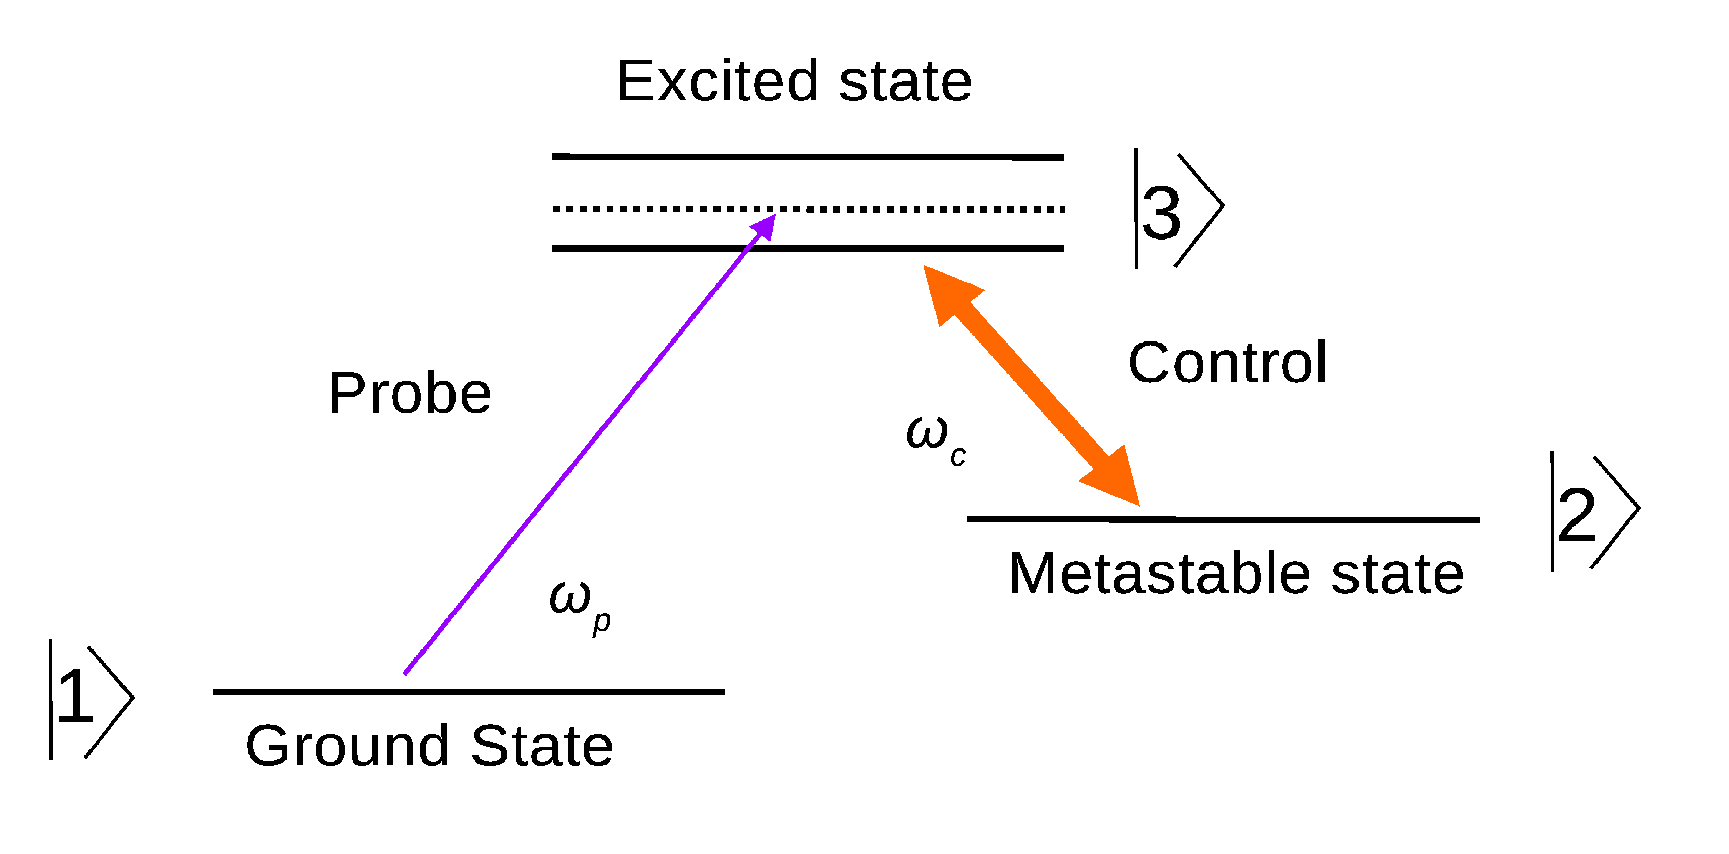
\includegraphics[scale=0.5]{EIT_3_level.eps}
\caption{A three-level atomic system where level three splits due to the presence of much stronger control laser field.}
\end{figure}

\subsection{Three Level Atoms}
To comprehend the occurrence of EIT, we focus on a Lambda-type three-level system shown in Fig. 3.1. In this system, we will discuss what happens quantum-mechanically for the effect of EIT, without disrupting the essence of classical phenomenons. The probability amplitudes of level $\ket{3}$ are driven by two terms in the system. One is the transition probability amplitude of the ground state $\ket{1}$ to the excited state and the other is the oppositely phased transition probability amplitude of the state $\ket{2}$ to the excited state. These both driving fields are opposite in signs but equal in magnitudes and have a frequency $\omega_{p}$ and are so balanced that probability amplitude of state $\ket{3}$ and the expected value of the amplitude of the sinusoidal motion at every frequency that has been applied is zero. 


One may ask how that opposite phase for a transition from the coherent states $\ket{1} \to \ket{2}$ along with the applied field $\omega_{c}$, makes absolute cancellation? Because we use the laser pulses that generate fast enough laser photons that the phase of transitions is maintained and is the correct phase for cancellation [2]. 

 
\section{Coupled Resonator Induced Transparency \\ (CRIT)}
We can observe EIT-like properties in various types of coupled-resonator systems. However, the scope of this thesis is limited to ring resonators systems only. The optical analog of EIT is referred to as Coupled Resonator Induced Transparency (CRIT). This kind of geometry (that we discussed in section 2.4) has been promising for a long time in the field of photonics. EIT analog can be explained based on destructive interference between two electromagnetic fields which circulates the ring resonator system. This system is mostly explained by classical wave travel [3].

\begin{figure}[h]
\centering
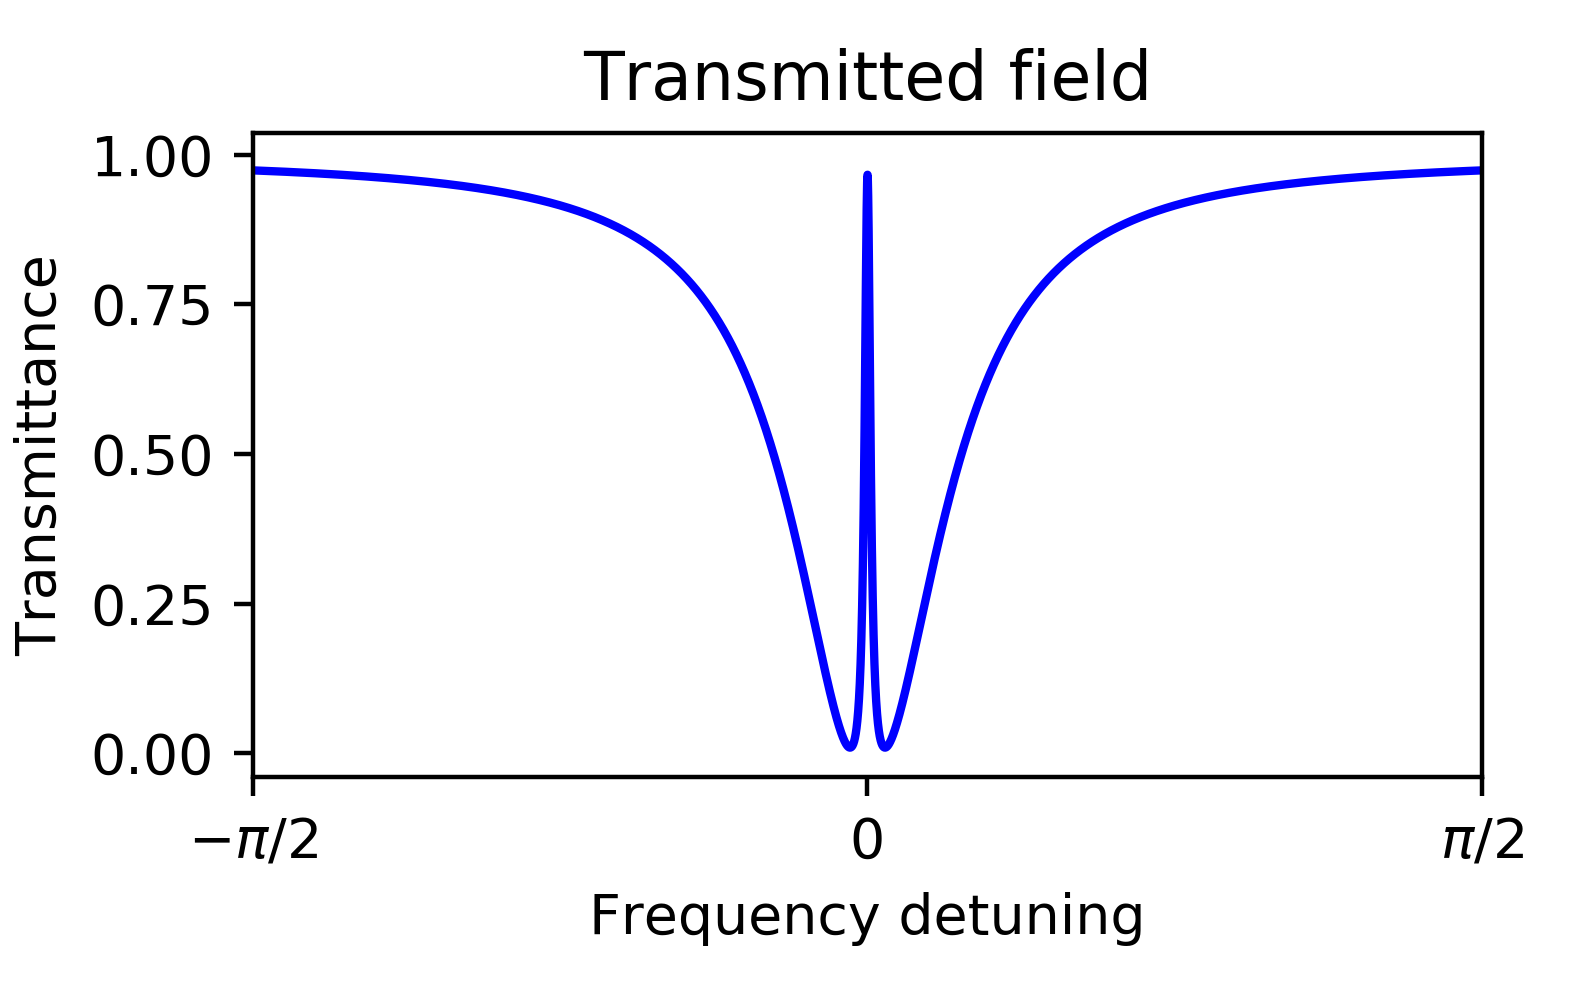
\includegraphics[scale=1]{coupled_ring_EIT1.png}
\caption{CRIT in a two ring resonator system.}
\end{figure}


The resonant incident light is coupled to the first ring through the evanescent field and circulates inside the ring and acquires a phase shift of 2$\pi$ after one round trip inside the optical cavity. The circulating light thus interferes constructively with the incoming light and a large intracavity is realized inside the resonator i.e. their phases match perfectly, then at those frequencies, there is a transparency window in the absorption spectrum i.e. a narrow dip, or we see a sharp peak in the transmission spectrum [2].


Figure 3.2 displays the reproduced plot of transmitted intensity vs round-trip phase $\phi$ in a coupled resonator system (as shown in Fig. 2.16 in chapter 2). The parameters used here $r_{1} = 0.9$ and $r_{2} = 0.999$ and attenuations $a_{1} = 0.88$ and $a_{2} = 0.9999$ for first and second resonator respectively. Reproduced from the original work on \textit{``Coupled resonator induced transparency"} [3] from 2004.


Now let us look at the phase response of such a coupled-resonator system. Figure 3.3 shows the effective phase of the entire system (red) and the phase of the transmitted field of the second resonator, in yellow. 

\begin{figure}[h]
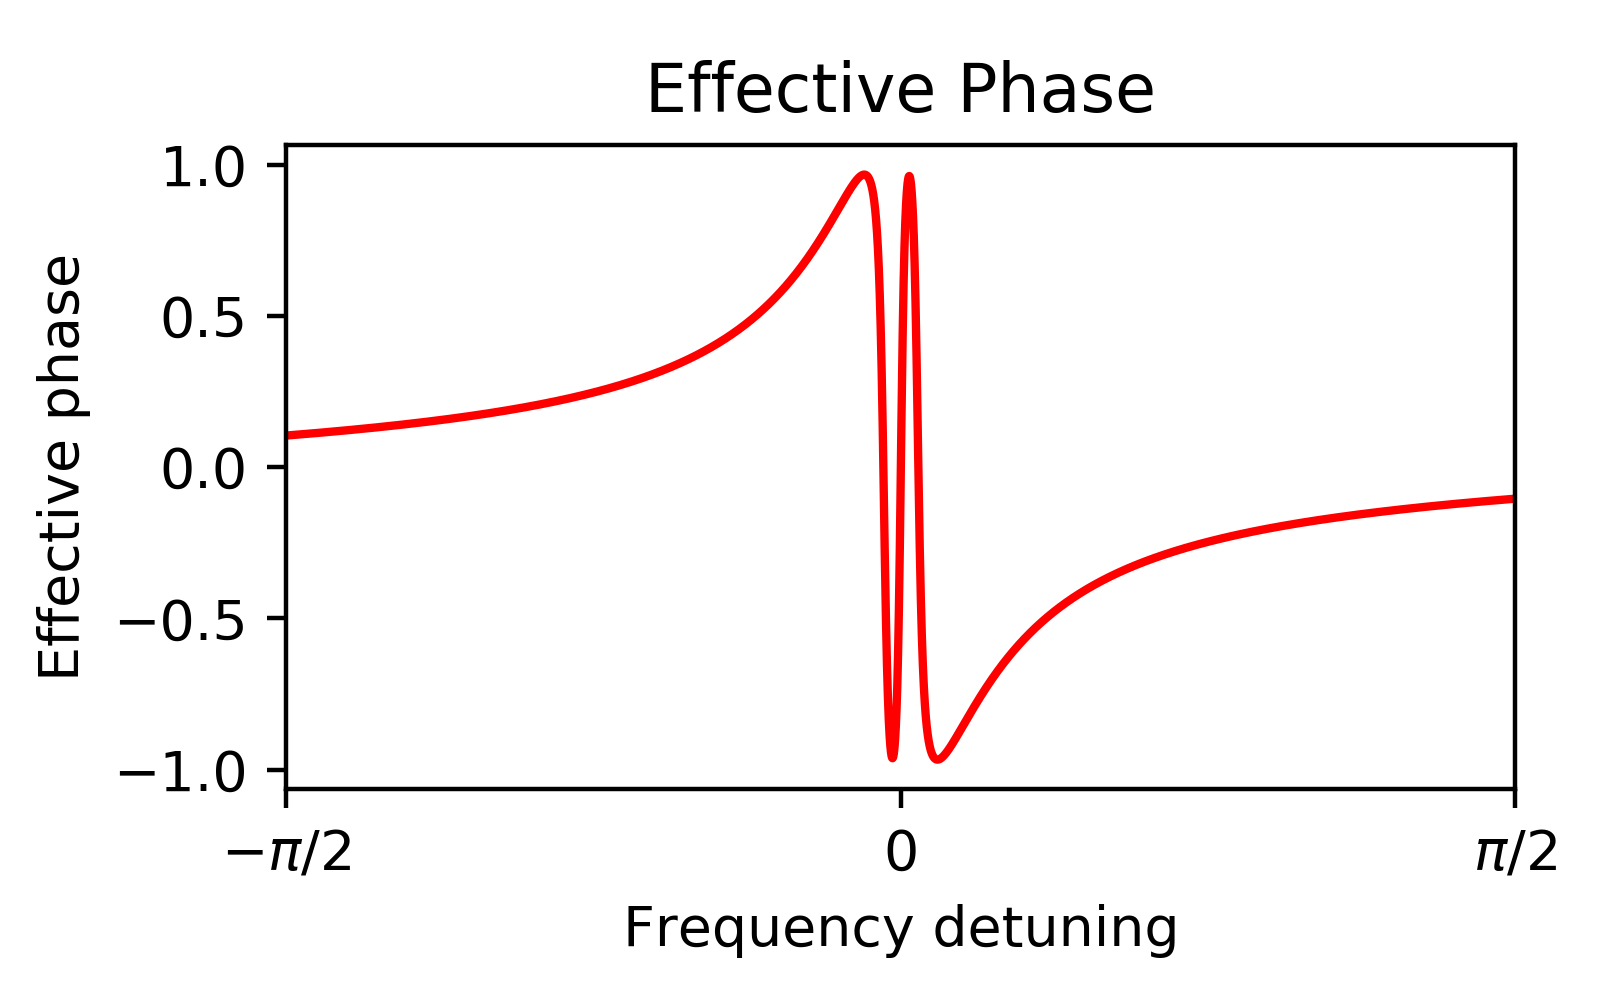
\includegraphics[scale=0.75]{coupled_ring_EIT1_phase.png}
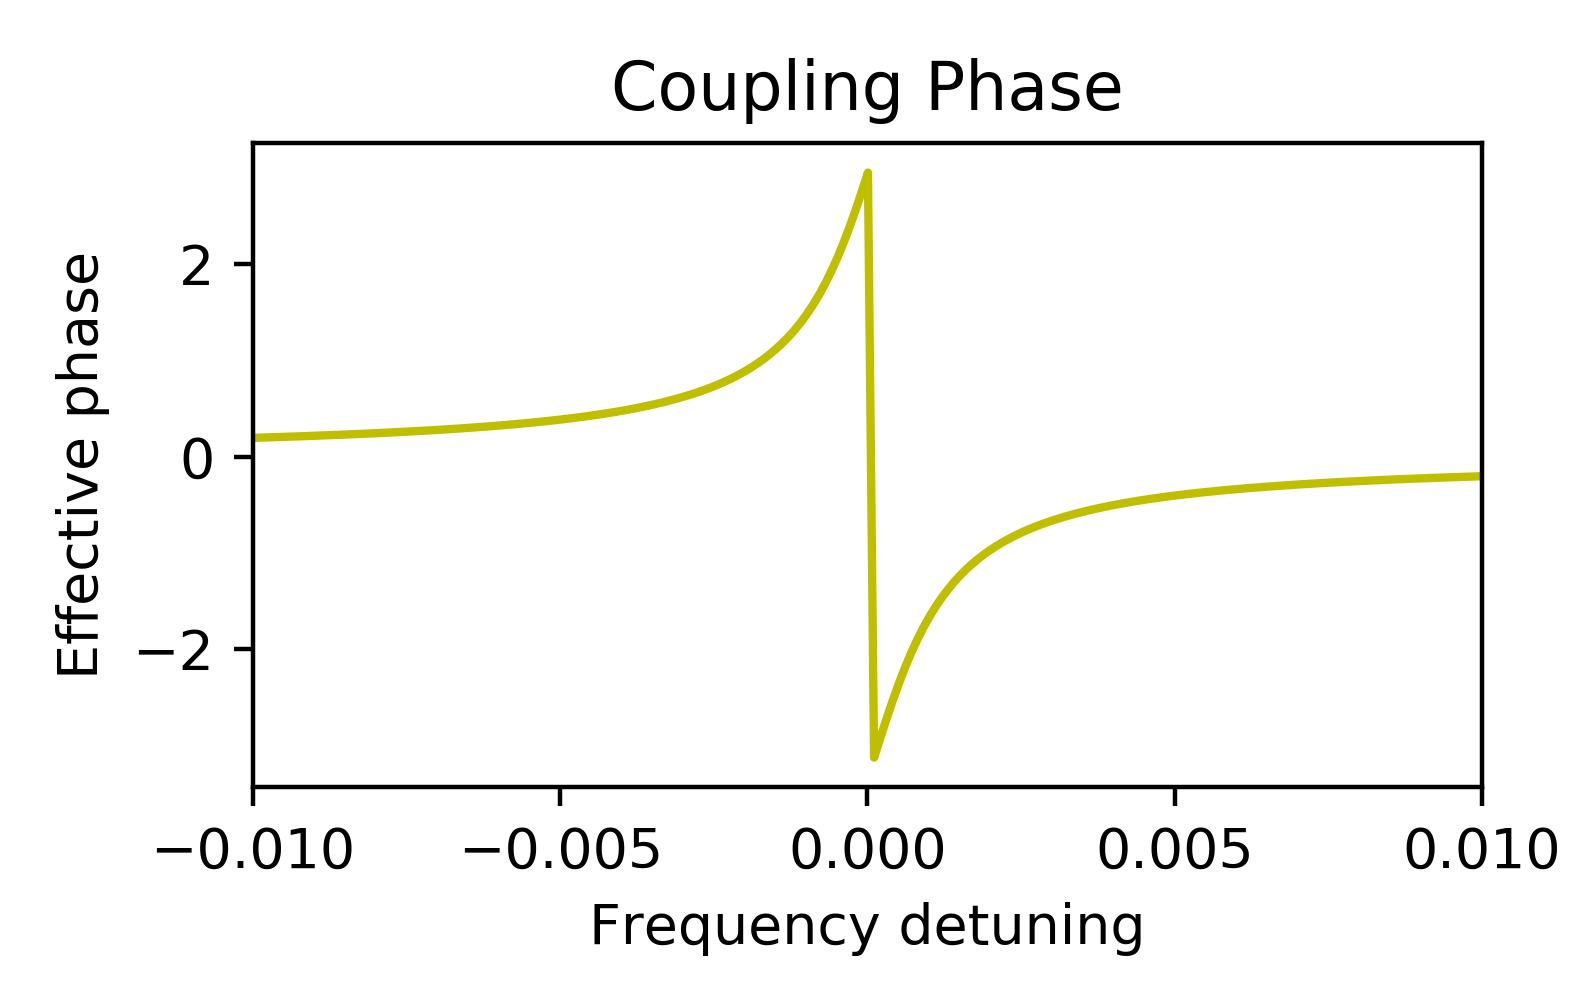
\includegraphics[scale=0.75]{coupled_ring_EIT1_coupling.png}
\caption{Effective phase of the system (red) and transmitted phase (yellow) vs round-trip internal phase.}
\end{figure}

Figure 3.4 shows the derivative of the phase of the system which gives us information about the group index and group velocity of the system. 

This value is directly related to the group index of the system. From the graph, we can see that there are negative group-index values for off-resonance regions and positive values on resonances. This informs us that we have superluminal light away from resonance while at resonance subluminal light is produced. 

\begin{equation}
\frac{1}{v_{g}} = \frac{n}{c} \frac{d\phi_{eff}}{d\omega}
\end{equation}

where, group index and group velocity are related by, 
\begin{align*}
n_{g} = \frac{c}{v_{g}}
\end{align*}

\begin{figure}[h]
\centering
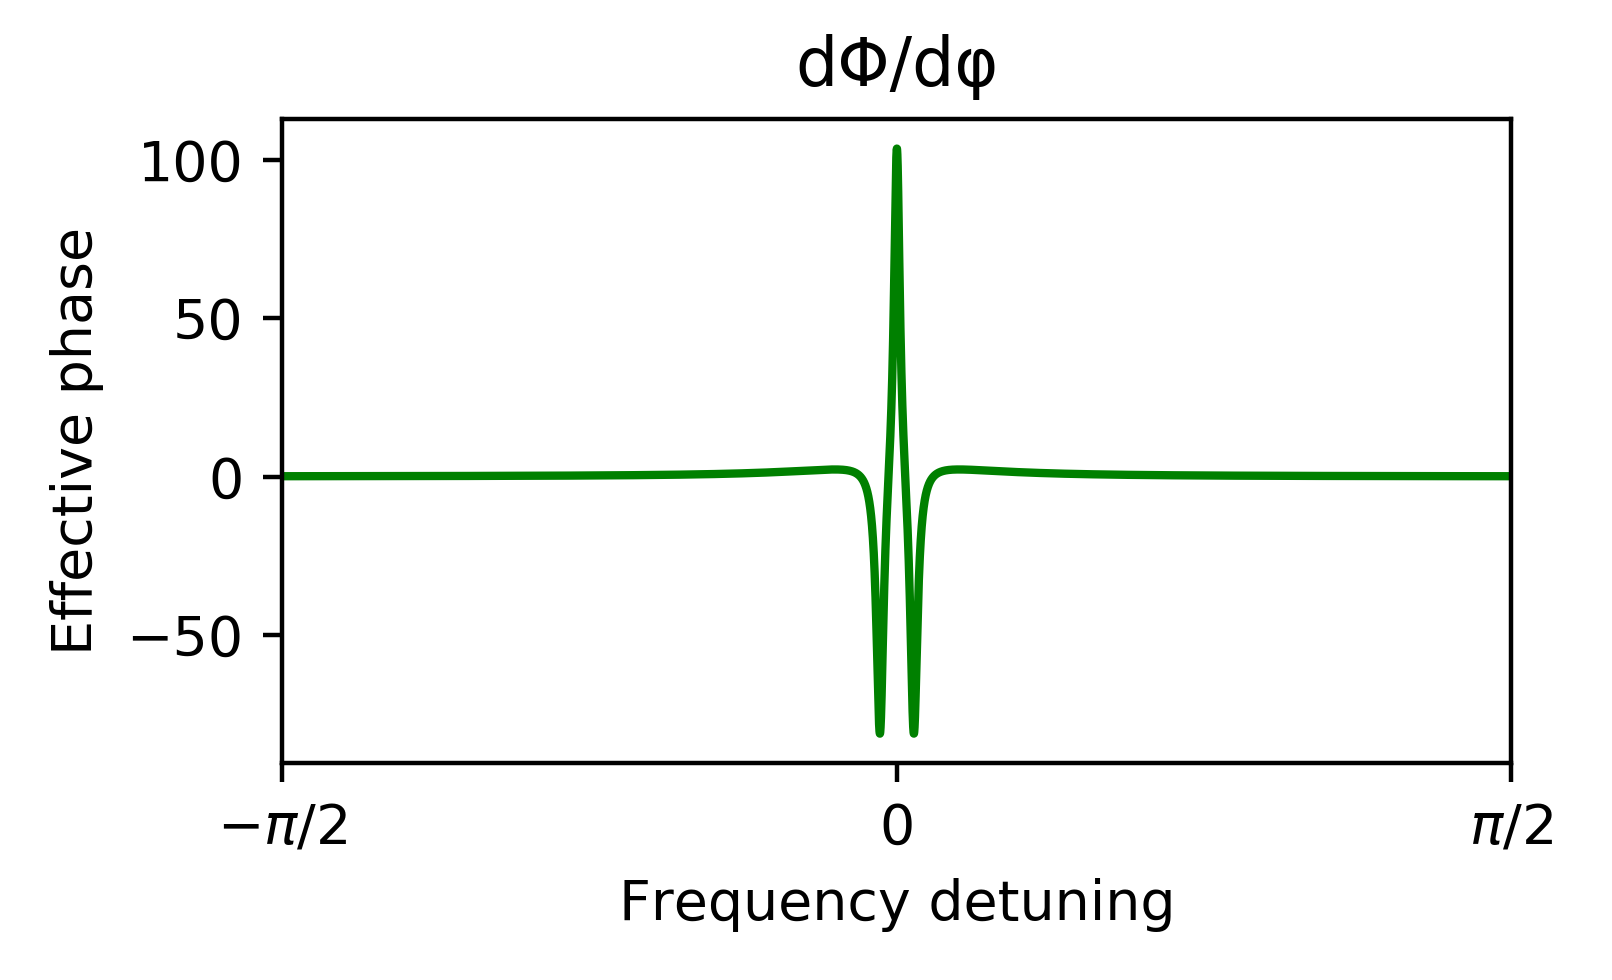
\includegraphics[scale=1]{coupled_ring_EIT1_deri.png}
\caption{Derivative of the transmitted phase of the system vs round trip phase.}
\end{figure}

\section{Electromagnetically Induced Absorption}
In contrast to EIT, in Electromagnetically Induced Absorption (EIA), constructive interference occurs between the transition probability amplitudes occurring across two transition pathways. This leads to a narrow dip at the center of the transmission dip in the spectrum of the system, known as Electromagnetically Induced Absorption (EIA) shown in Fig. 3.5. As a whole, EIA is not a very well understood phenomenon and its explanation lacks the true essence.

\begin{figure}[h]
\centering
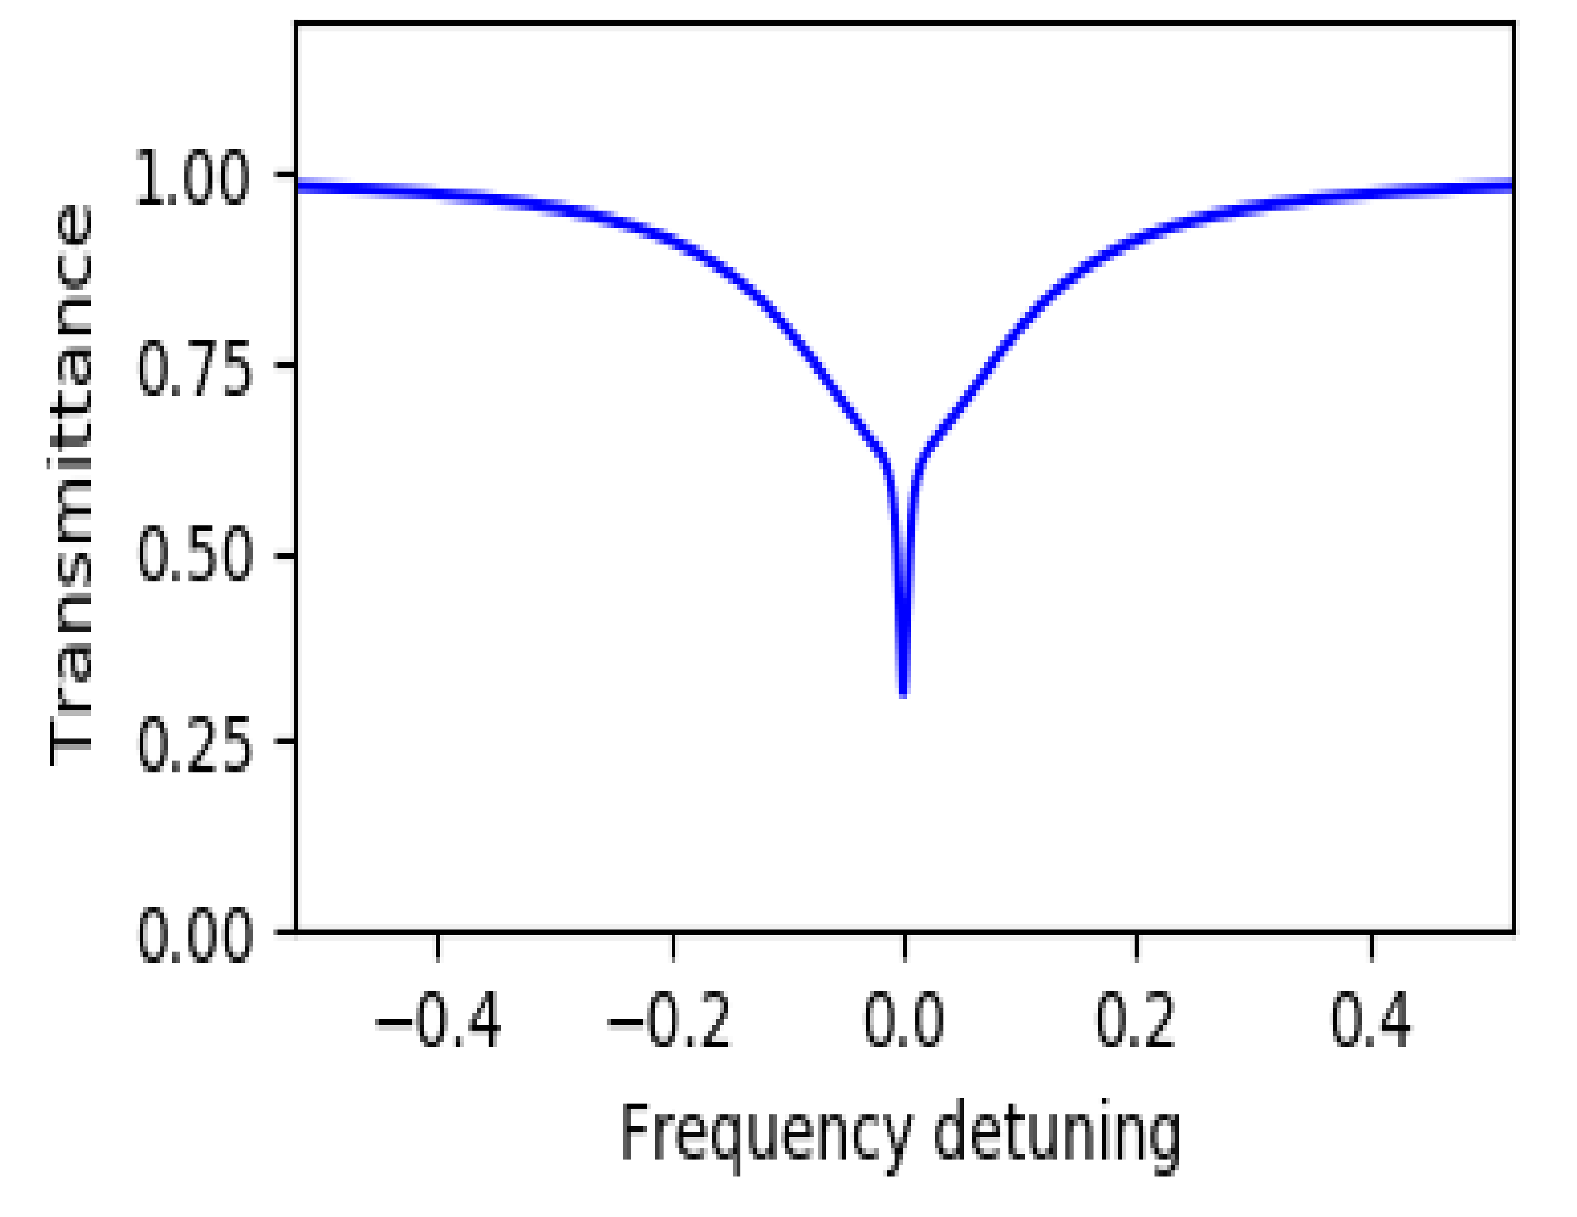
\includegraphics[width=0.5\textwidth]{EIA_basic.eps}
\caption{CRIA in a coupled two ring resonator system.}
\end{figure}

\section{Coupled Resonator Induced Absorption} 
 
Coupled resonator system as discussed above also displays EIA-like effect. The optical analog of EIA is known as Coupled Resonator Induced Absorption (CRIA). CRIA can give us both fast light and slow light, most of the light leading to a different set of broad applications. The system discussed below is again a two-ring resonator system as above and we will again follow the same procedure. Fig. 3.5 displays the CRIA in ring resonator system with coupling parameters as $r_{1} = 0.8998$ and $r_{2} = 0.9998$


\subsection{CRIT in a Passive System}
As before, now we are going to observe what changes does the system has when we introduce gain in it. For convenience, we will first see the passive results for a system and then introduce gain in either in second resonator or first resonator and then introducing gain in both of the resonators. This can be introduced by pumping some monochromatic light source or a laser, in either one of the rings which will drastically compensate the losses inside the resonator and will increase the overall output transmission of the system even above the incident light source. The system parameters are as follows, $r_{1} = 0.9889$ and $r_{2} = 0.9998$ with $Q_{1} = 1\times10^{5}$ and $Q_{2} = 1\times10^{6}$ for first and second resonator respectively (Fig. 3.6). 

\section{Gain-controlled CRIT in coupled resonator}
We observe EIT in a coupled two resonator system, the transmission and effective phase of the system is shown in Fig. 3.6 displaying normal dispersion meaning slow light in the system.

\begin{figure}[h]
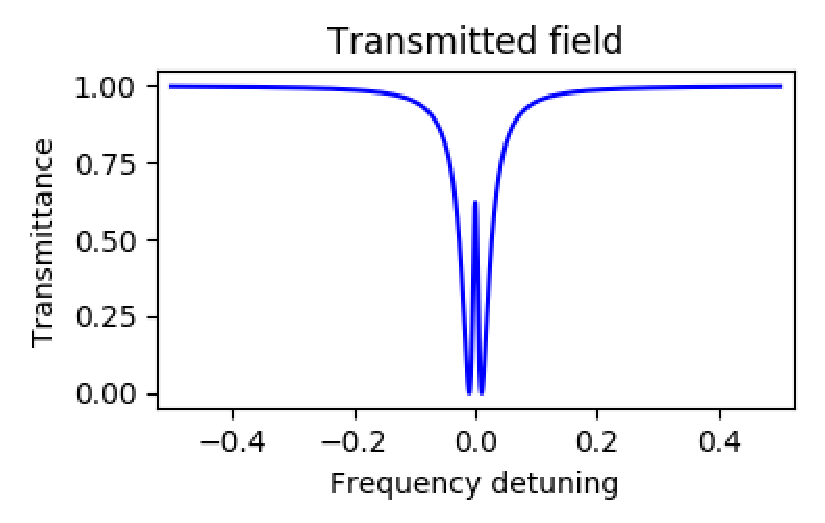
\includegraphics[scale=0.5]{EIT_1.eps}
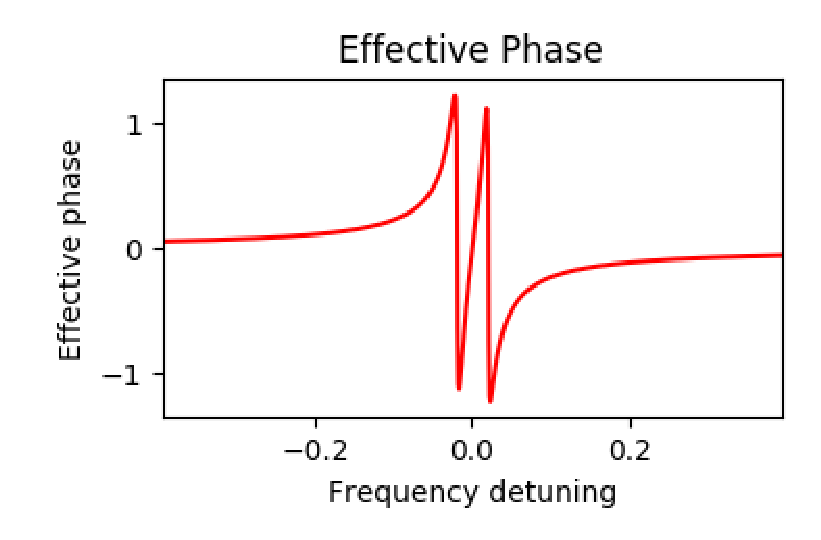
\includegraphics[scale=0.5]{EIT_phase.eps}
\caption{CRIT with its effective phase in a passive resonator system.}
\end{figure}

\subsection{Introducing Gain Only In Second Resonator}
Now we will activate gain in the second resonator, which has higher Q-factor (labeled 2 in Fig. 3.7). We increase the gain to compensate for the intrinsic losses, denoted by $\alpha_{i}$, which is directly related to the Q-factor of the resonator. The transmission peak of the EIT starts to rise gradually to $g$, the gain coefficient is increased. The peak rises towards unity up till $g_{2} \to \alpha_{i,2}$, where alpha is the attenuation constant for intrinsic loss. 

\begin{figure}[h]
\centering
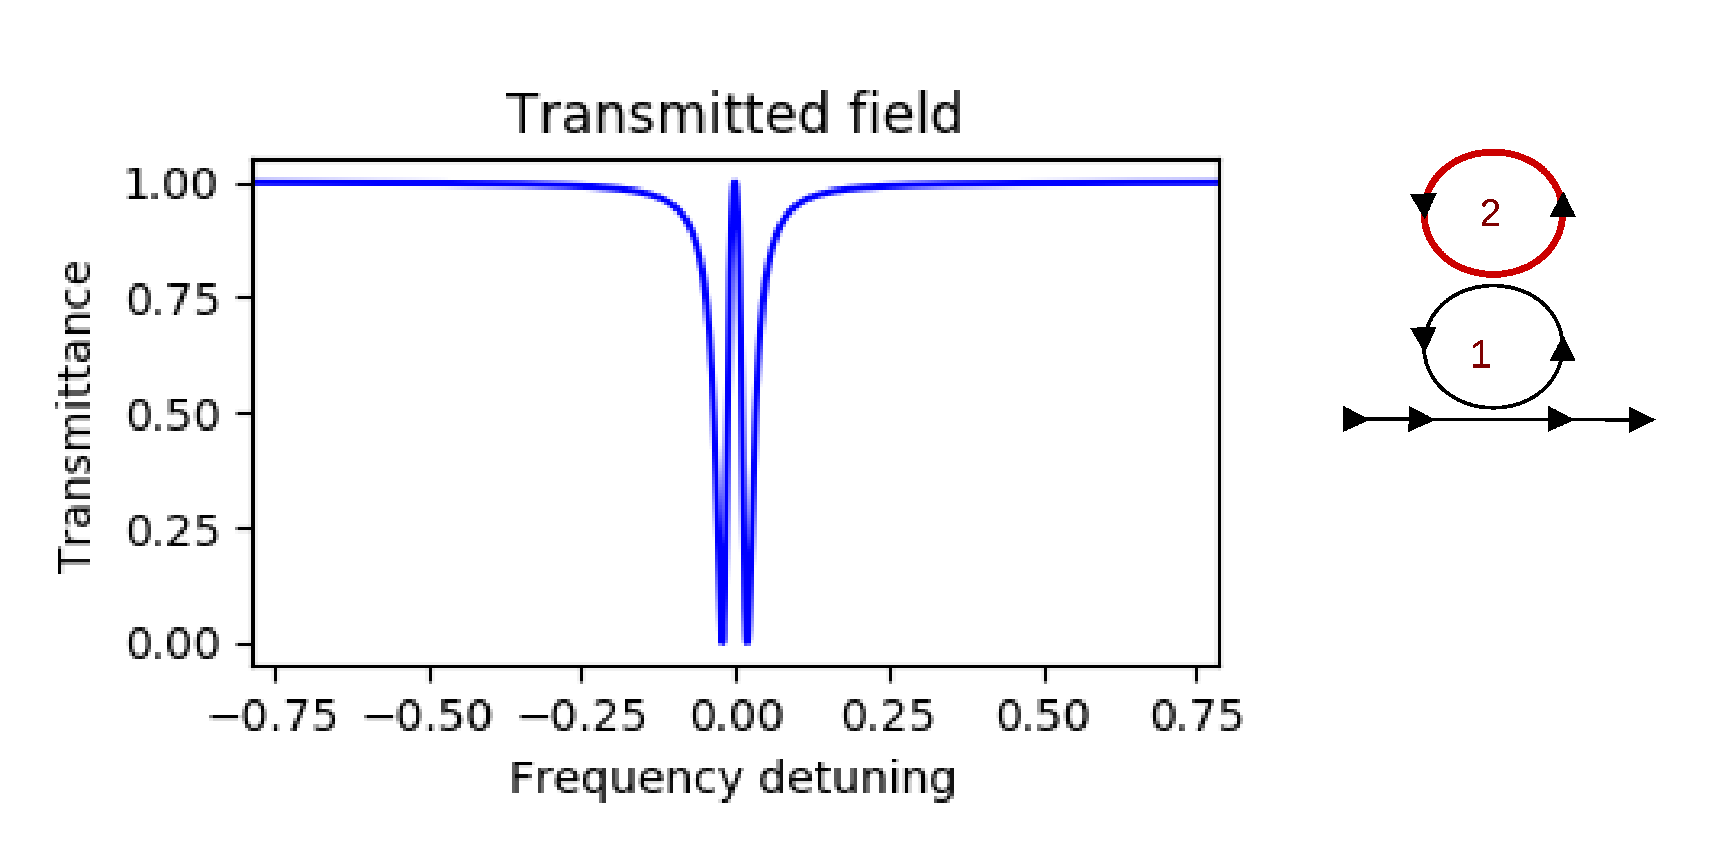
\includegraphics[scale=0.5]{EIT_gain2.eps}
\caption{CRIT in an active coupled resonator system.}
\end{figure}

When gain coefficient equals the intrinsic loss coefficient, i.e. $g = \alpha_{i}$, the peak of the transmission touches the unity on the graph this implies that all of the incident light is verily being transmitted the other side i.e. the medium has become completely transparent for resonant frequencies. This means that we have now compensated for all the losses inside the system which are intrinsic. When this happens, we see an abrupt change in the effective phase of the system. This system now gives us anomalous dispersion on-resonance meaning we get fast light in EIT (Fig. 3.8). 

To get a brief idea of what is happening, I have also calculated the group index of the system. In this case, we receive negative values for the group index $n_{g}$ on resonance. Fig. 3.9 displays the group index for this particular case.


\begin{figure}[h]
\centering
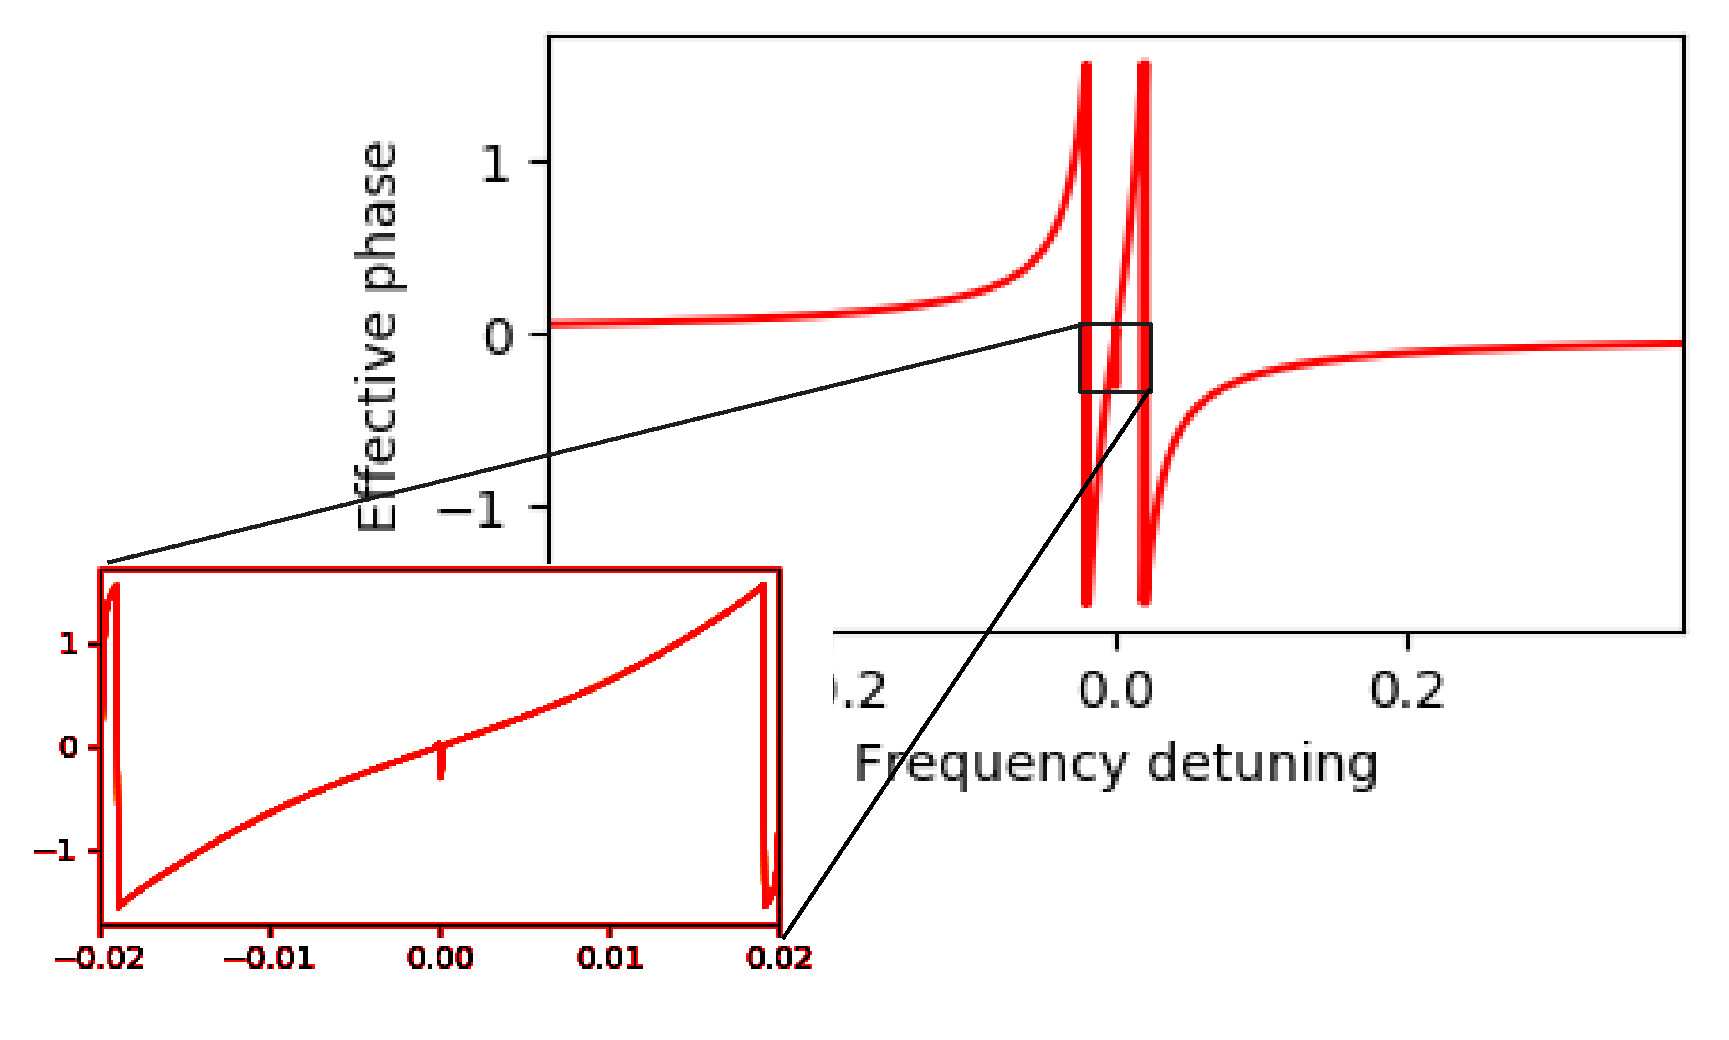
\includegraphics[scale=0.30]{EIT_gain2_phase.eps}
\caption{Effective phase of CRIT in an active coupled resonator system. Magnified view of phase near resonance frequency is shown.}
\end{figure}

     
\begin{figure}[h]
\centering
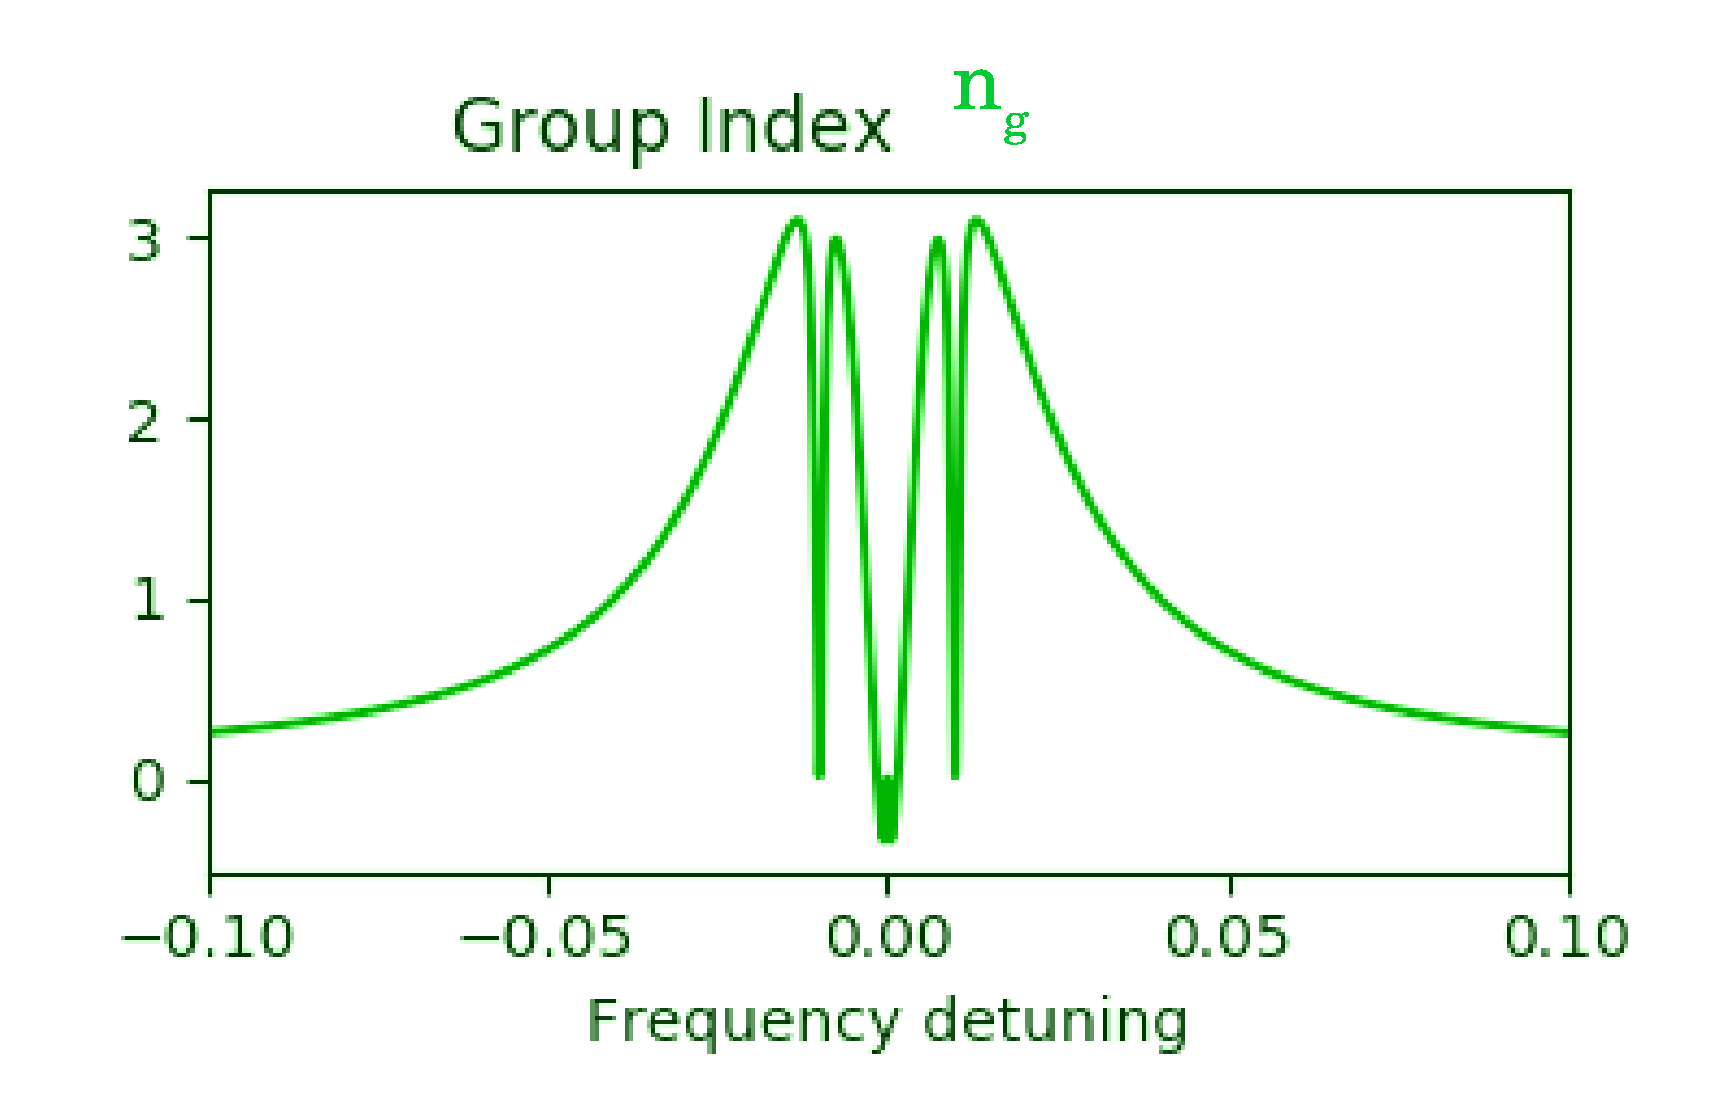
\includegraphics[scale=0.30]{EIT_gain2_ng.eps}
\caption{Group index of an active resonator system showing negative values on resonant frequency.}
\end{figure}


\subsection{Introducing Gain Only In First Resonator}
Now we will activate gain in the first resonator (labeled 1), which has lower Q-factor in comparison to the second resonator. The spectrum of the EIT starts to rise and displays a hanging EIT. (Fig. 3.10)

\begin{figure}[h]
\centering
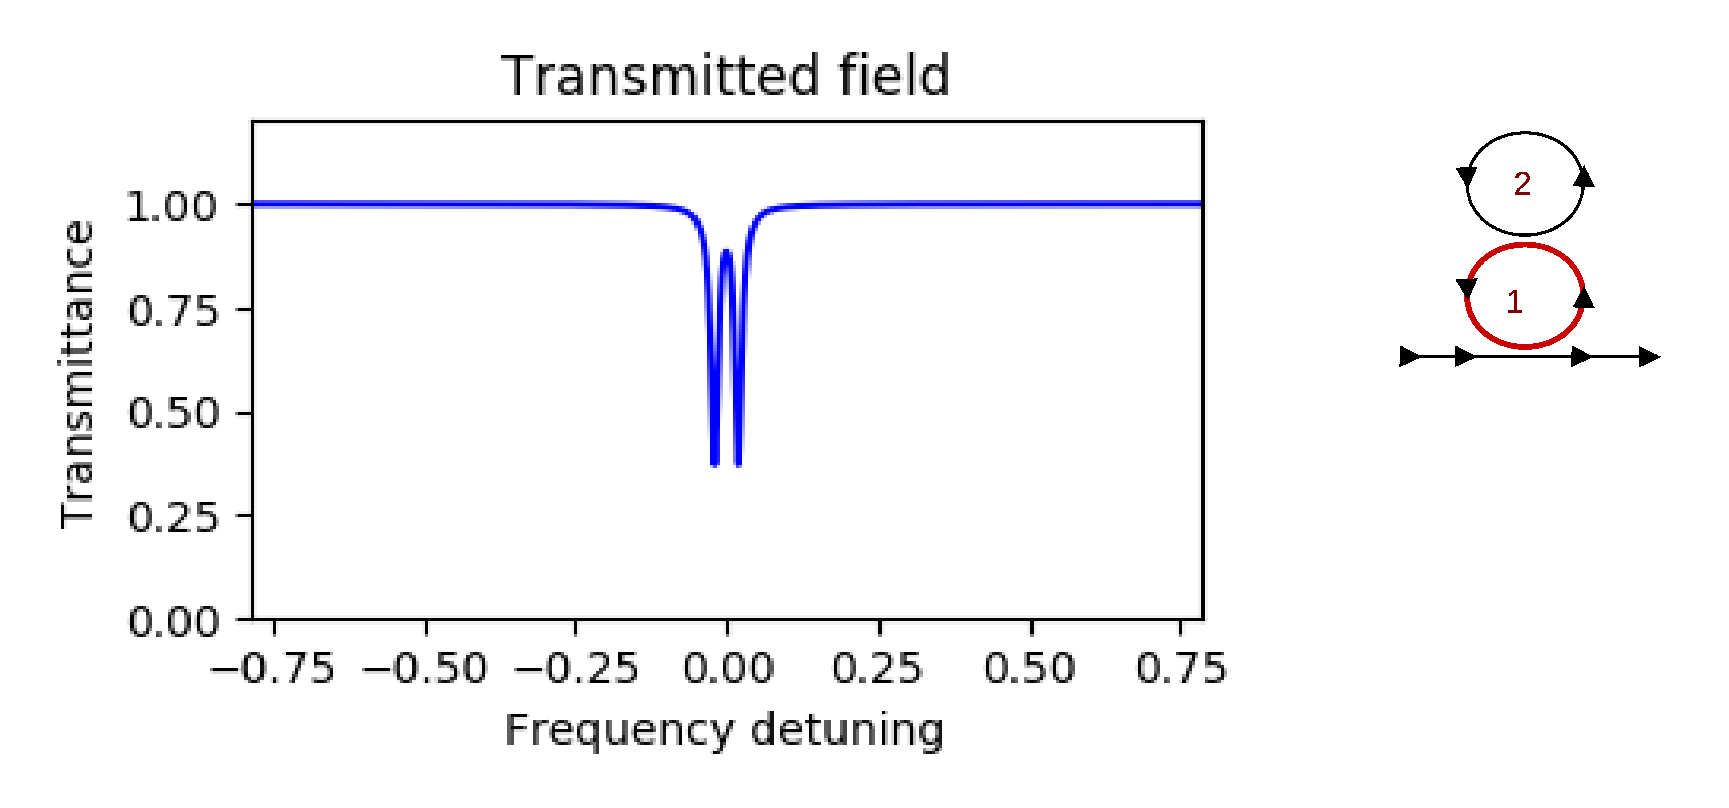
\includegraphics[scale=0.35]{EIT_gain1.eps}
\caption{CRIT of the two resonator system with gain activated in resonantor 1.}
\end{figure}

The effective phase of the system remains similar to a passive resonator, displaying normal dispersion (slow light). The index value on resonance calculated to be about $\approx 76.2$ which shows that light has been slowed down only marginally for this case (Fig. 3.11). 

\begin{figure}[h]
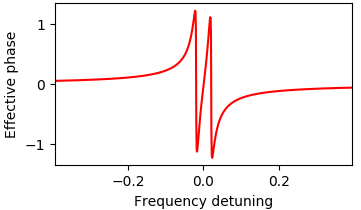
\includegraphics[scale=0.5]{EIT_gain1_phase.png}
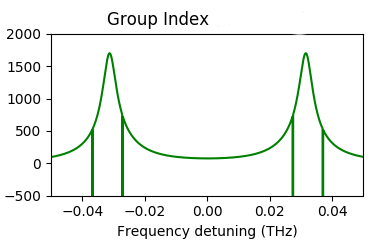
\includegraphics[scale=0.5]{EIT_gain1_ng.png}
\caption{Effective phase shows normal dispersion (in red) and group index $n_{g}$ shown in green.}
\end{figure}


\subsection{Introducing Gain In Both Resonators}
Now we will activate gain in both of the resonators simultaneously such that the ratio of the gain coefficients, $g_{1}$ and $g_{2}$, are the same. We observe that the peak of the EIT, as well as the whole transmission, starts to rise towards unity as $g_{1,2} \to \alpha_{i}$ (Fig. 3.12). The EIT transmission window also narrows down gradually.

\begin{figure}[h]
\centering
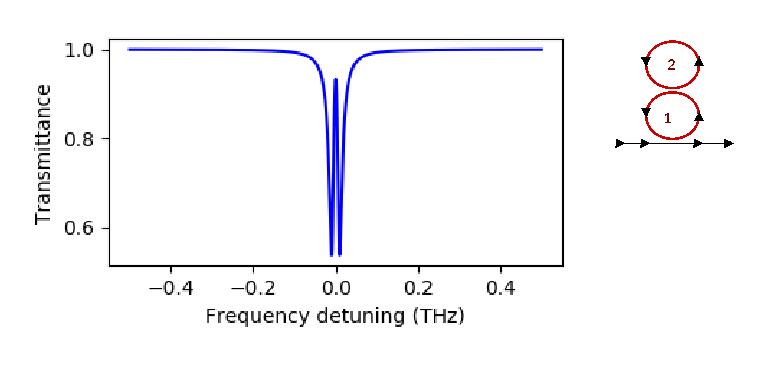
\includegraphics[scale=0.70]{EIT_gain12.eps}
\caption{Transmission graph of two resonator system with gain activated in both.}
\end{figure}

The effective phase of the system shows rather distinct curves which are basically due to the artifacts in the system or computation errors. The on-resonance information tells us that we have normal dispersion and positive group index about $\approx 766.5$ (Fig. 3.13). 

\begin{figure}[h]
\centering
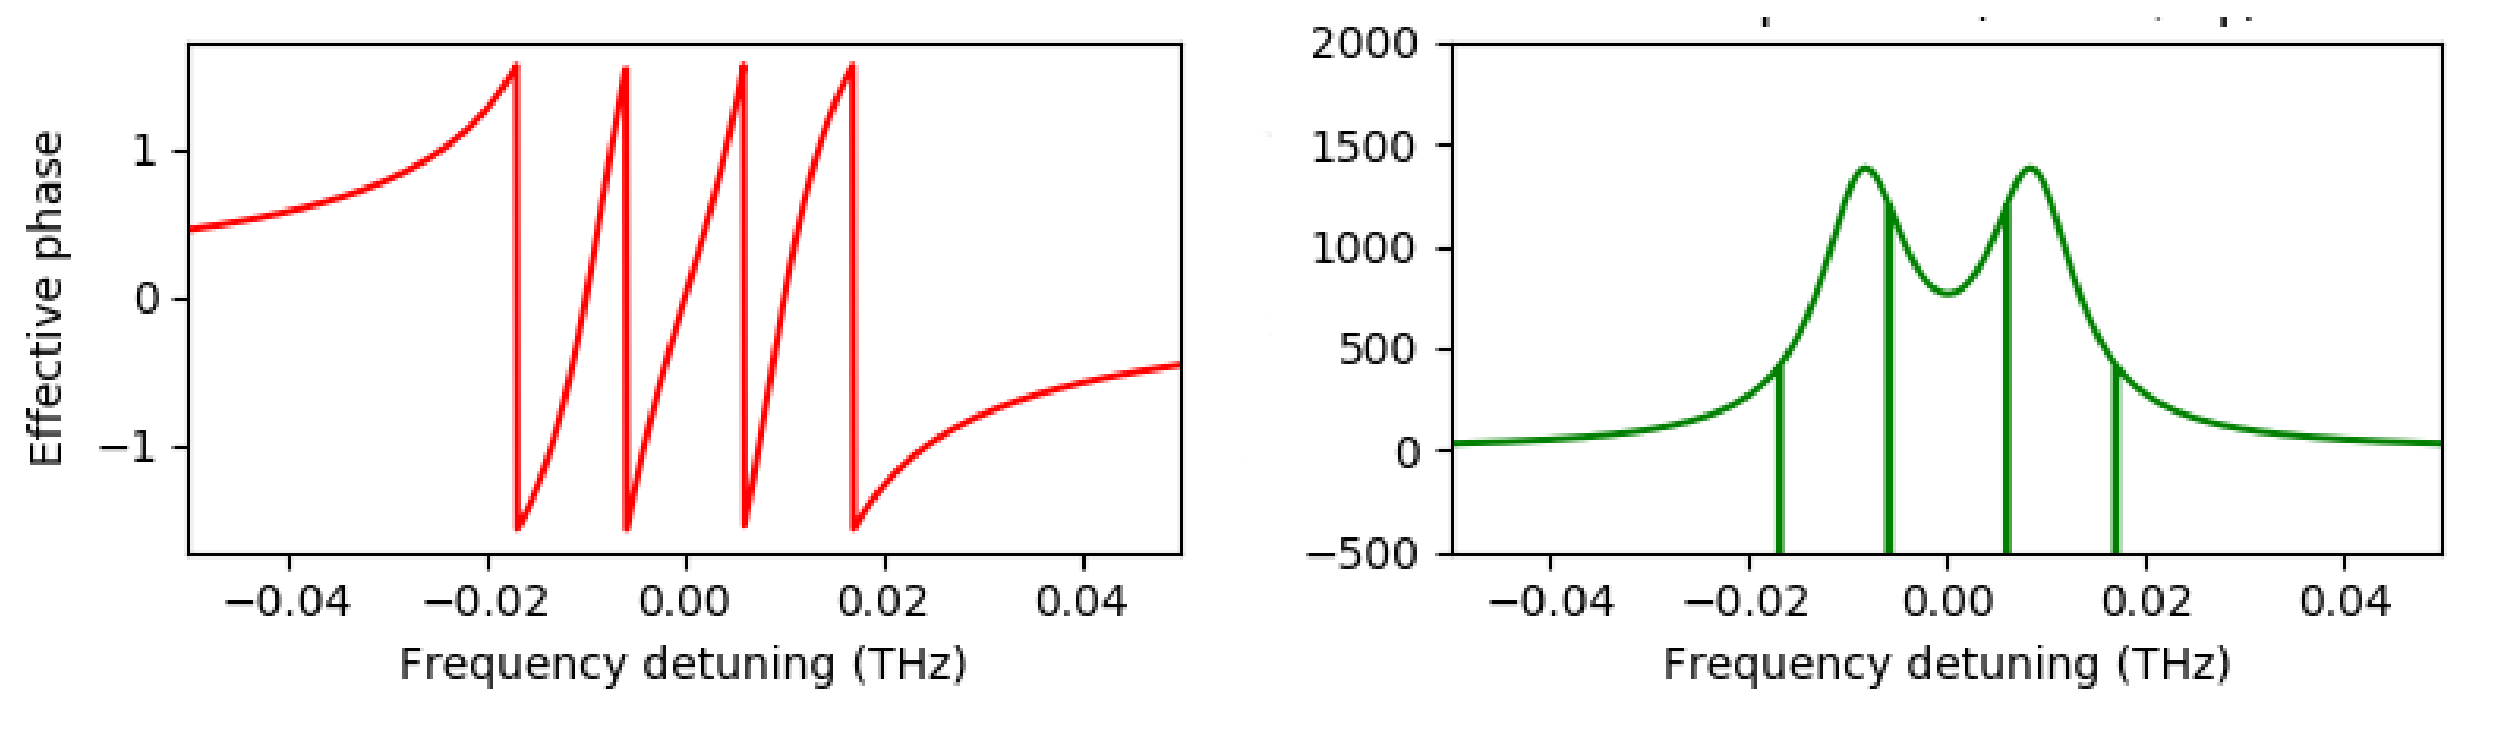
\includegraphics[scale=0.35]{EIT_gain12_phase.eps}
\caption{Phase and group index of a resonator system with gain in both resonators.}
\end{figure}

When the gain coefficient $g$ becomes greater than the intrinsic loss coefficient $\alpha_{i}$, then the whole transmission graph flips about the horizontal axis and we now see a distinct spectrum with a reversed EIT shown in Fig. 3.14.

\begin{figure}[h]
\centering
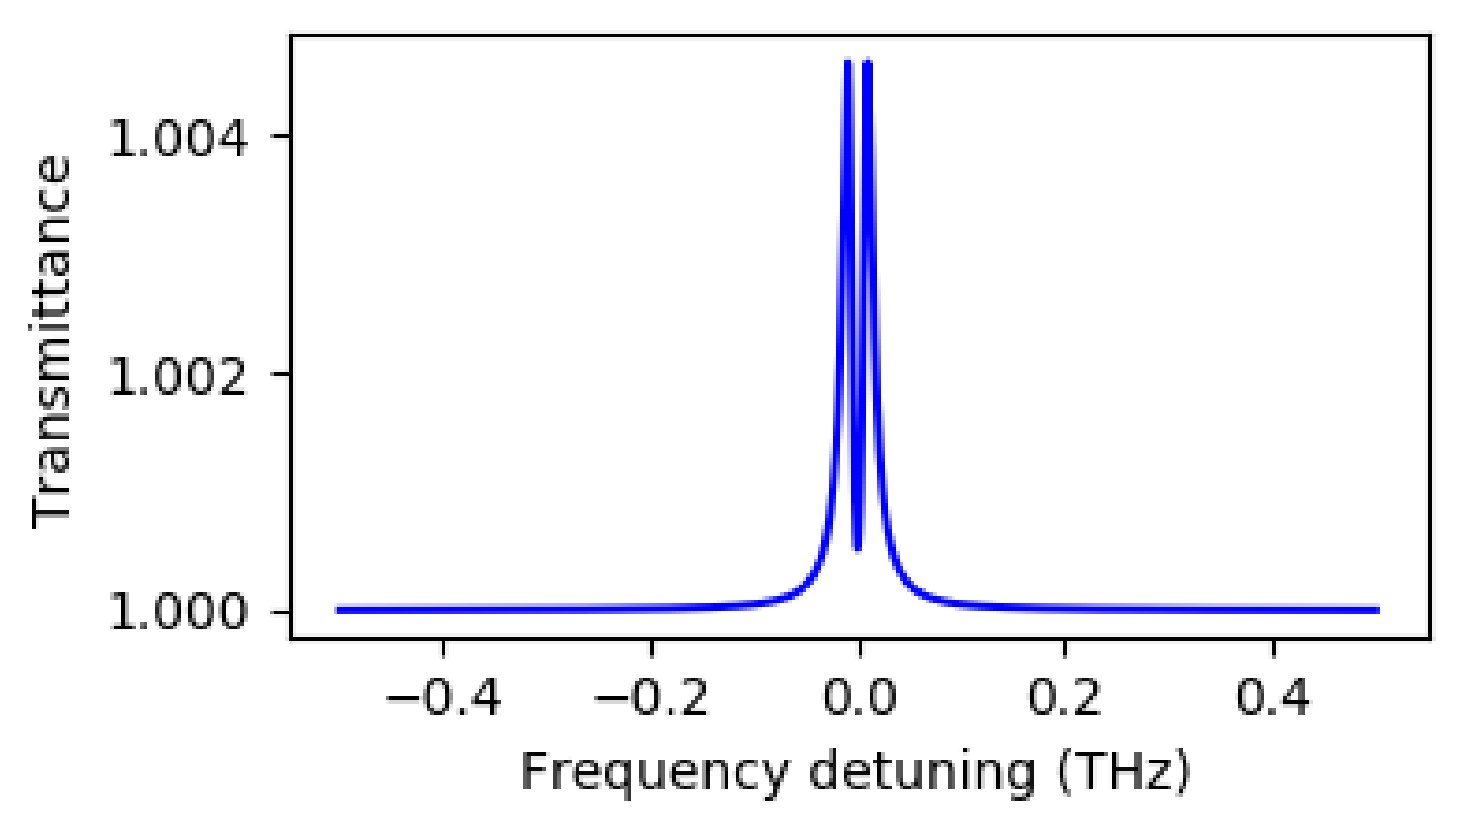
\includegraphics[scale=0.35]{EIT_gain12b.eps}
\caption{Flipping of the EIT spectrum when gain coefficient is larger than the attenuation coefficient.}
\end{figure}

This flipping of the transmission does not affect the dispersion of the medium. This means the effective phase and the group index of the system are similar in this case. However, we now have a transmission peak which is above unity. This shows that due to gain, intrinsic losses have been compensated and a transparent coupled resonator system is achieved.


  

\section{Gain-controlled CRIA in Coupled Resonators}
Now we will observe the behavior of the transmission spectrum of CRIA when we introduce gain in it. Similarly, first we are going to activate again in the second resonator, then into the first resonator and in last we activate and increase gain in both resonators simultaneously. 

\subsection{CRIA With Slow Light in Passive Coupled Resonators}
We will first examine the response of the CRIA (Fig. 3.5) in a passive medium with having normal dispersion. shown in Fig. 3.15, with its group index.

\begin{figure}[h]
\centering
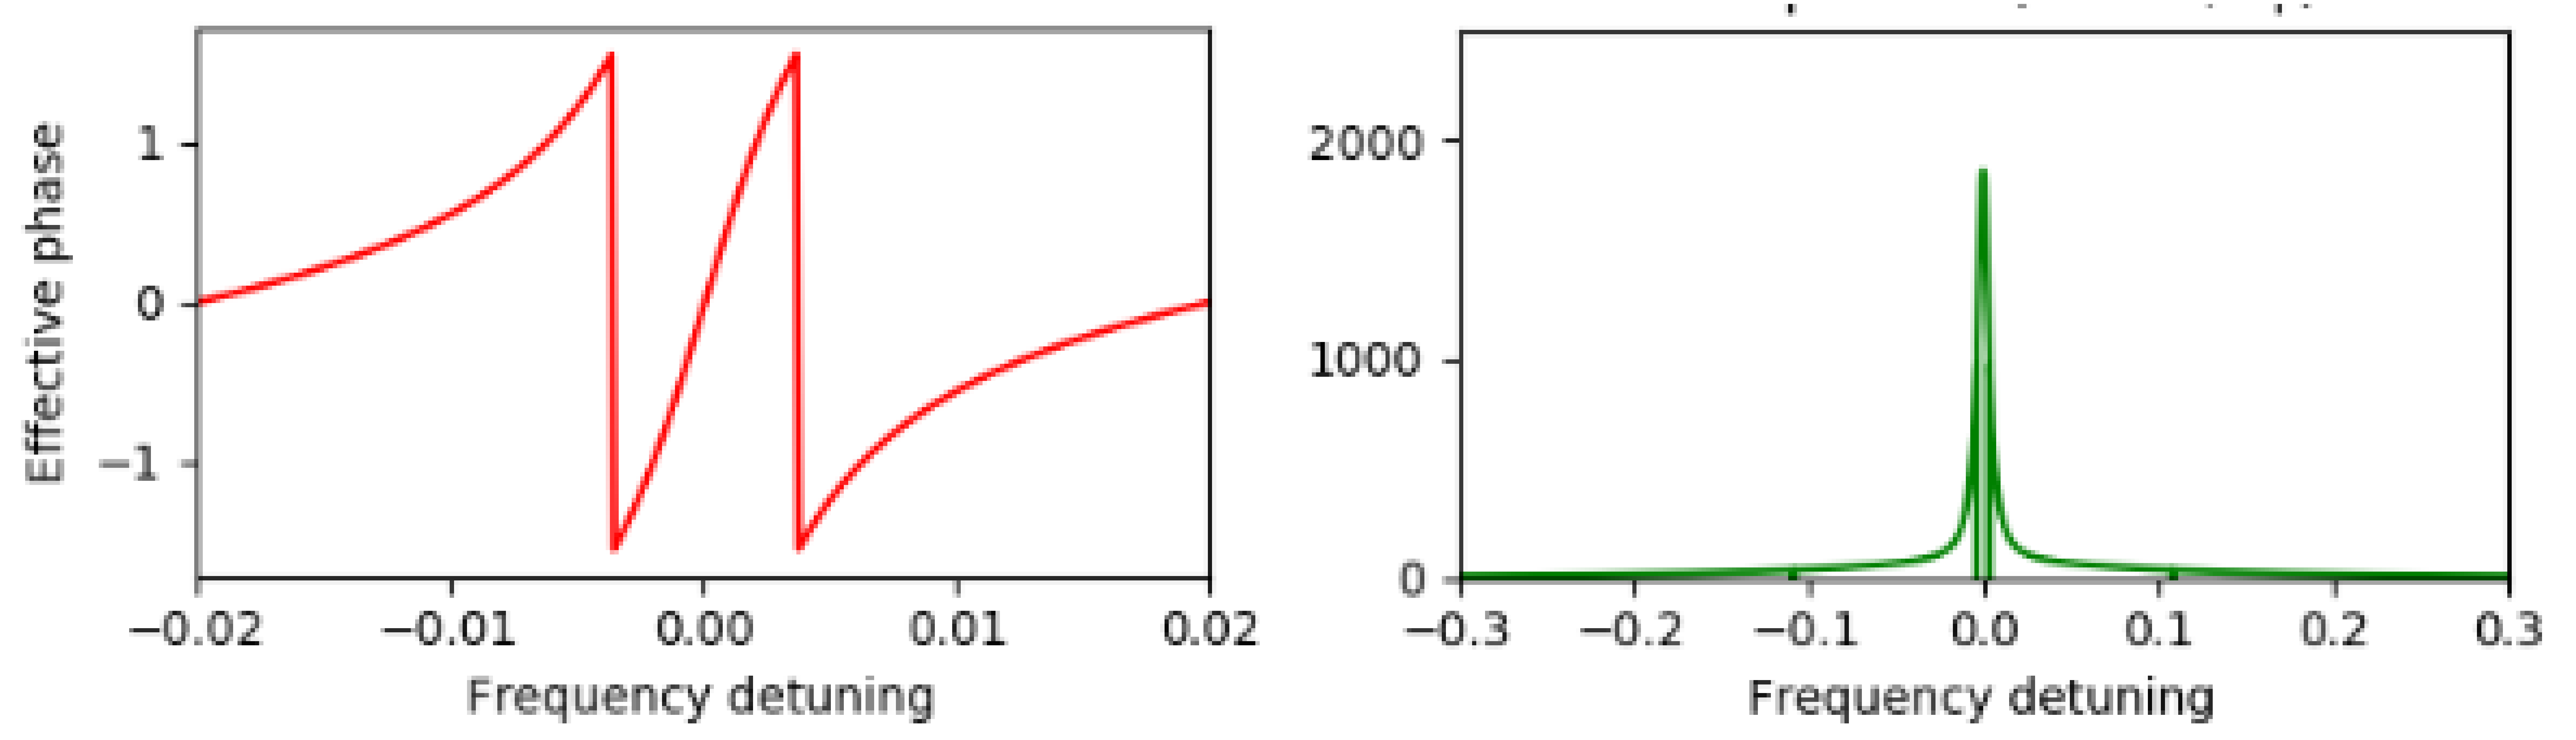
\includegraphics[width=1\textwidth]{EIA_gain_phase1.eps}
\caption{Phase and group index of CRIA.}
\end{figure}
  
\subsection{Introducing Gain Only In Second Resonator}
Now we activate gain in the second resonator such that $g \leqslant \alpha_{i}$.  When the gain becomes closer to the value of $\alpha_{i}$ ($g \to \alpha_{i}$), the EIA spectrum changes into EIT type transmission (Fig. 3.16).

\begin{figure}[h]
\centering
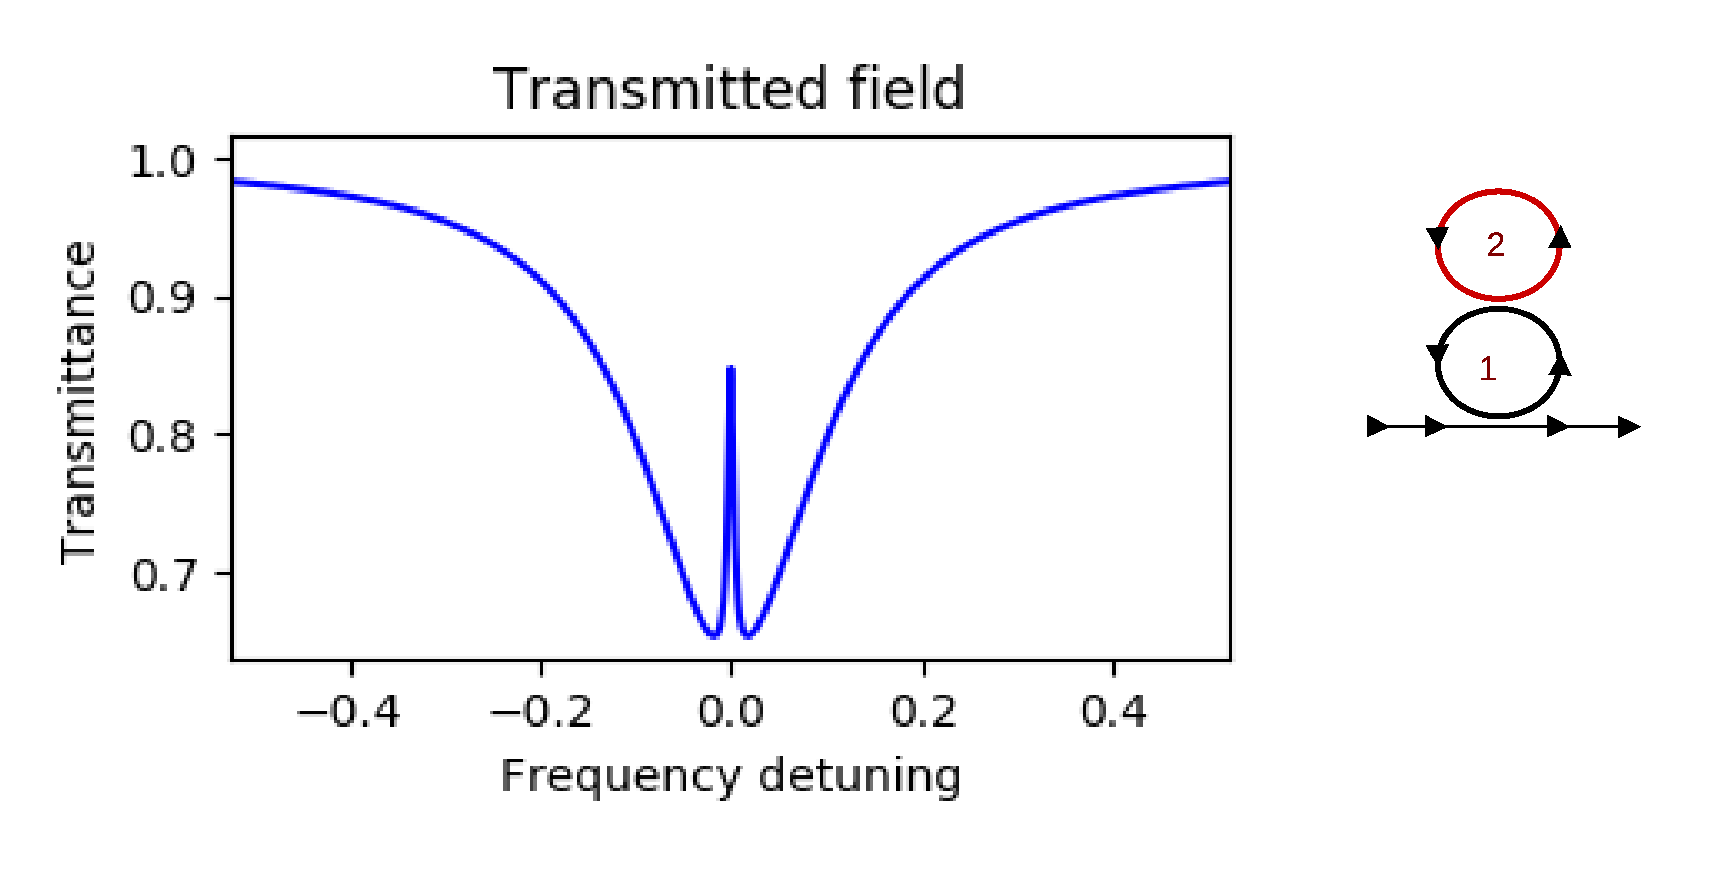
\includegraphics[scale=0.30]{EIA_to_EIT.eps}
\caption{CRIA dip changes from Fig. 3.5 into an CRIT type transmission when gain is introduced in second resonator.}
\end{figure}

The effective transmission phase changes from normal dispersion to anomalous dispersion. Corresponding group index displays a negative value of $n_{g} \approx -4505$ at resonance, implying a negative group delay and therefore, superluminal light (Fig. 3.17). Thus EIT which, in a passive coupled resonator system, always yields slow light, now enables superluminal (fast light) group velocities of resonant frequencies.

\begin{figure}[h]
\centering
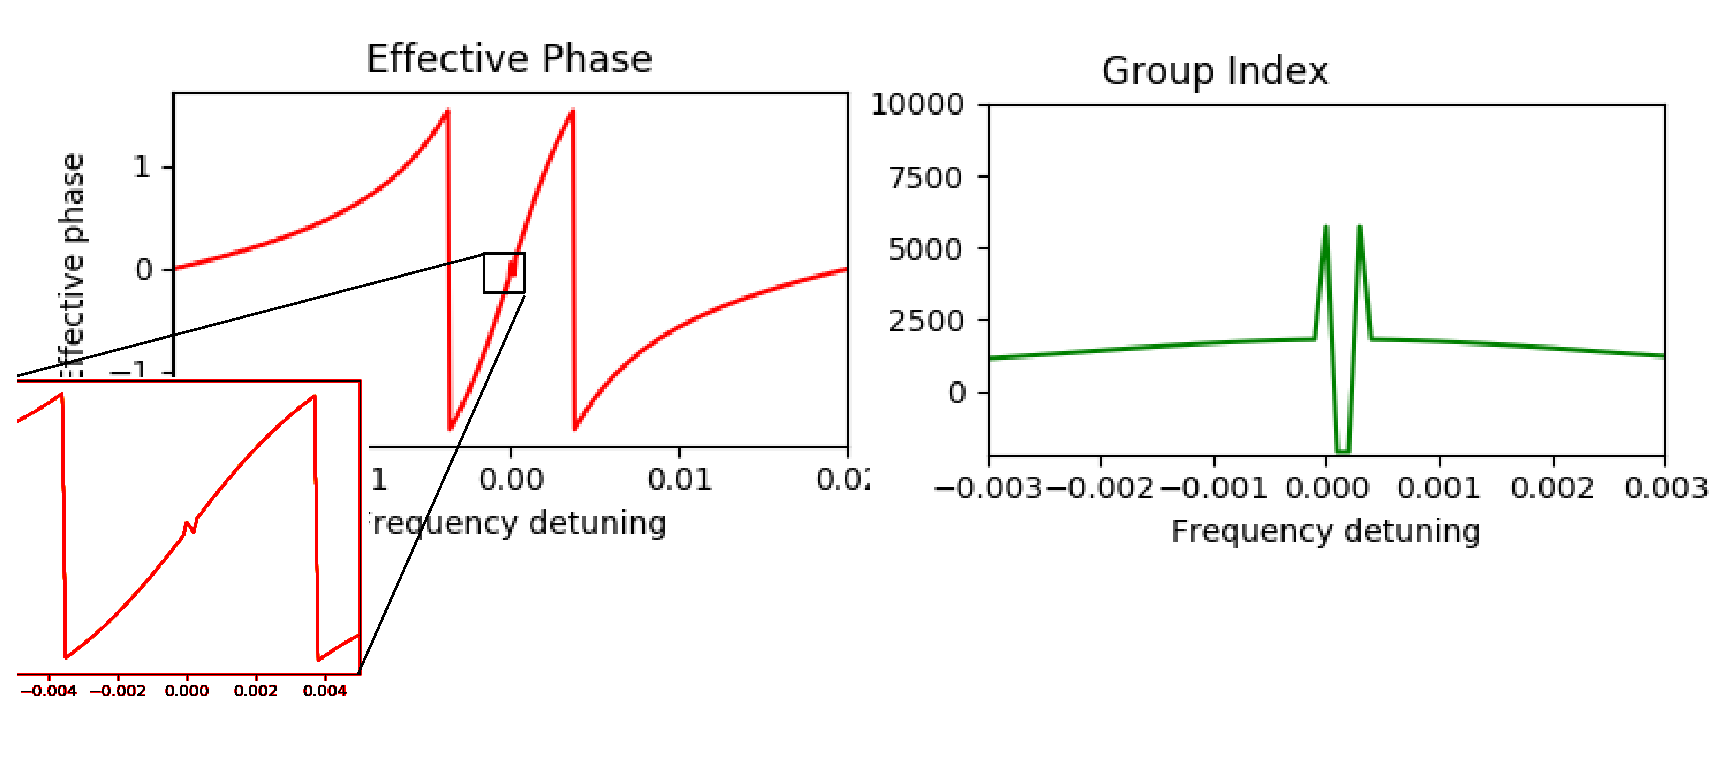
\includegraphics[scale=0.45]{EIA_to_EIT_phase.eps}
\caption{Phase of the system showing anomalous dispersion on resonance (zoomed) and group index showing negative values.}
\end{figure}

\subsection{Introducing Gain Only In First Resonator}
Now we activate gain in the first resonator (labeled 1 in Fig. 3.18) and observes that the EIA resonance narrows down and eventually becomes a sharp transmission dip. Fig. 3.18. Corresponding transmission phase and group index reveal normal dispersion and slow light (Fig. 3.19).


\begin{figure}[h]
\centering
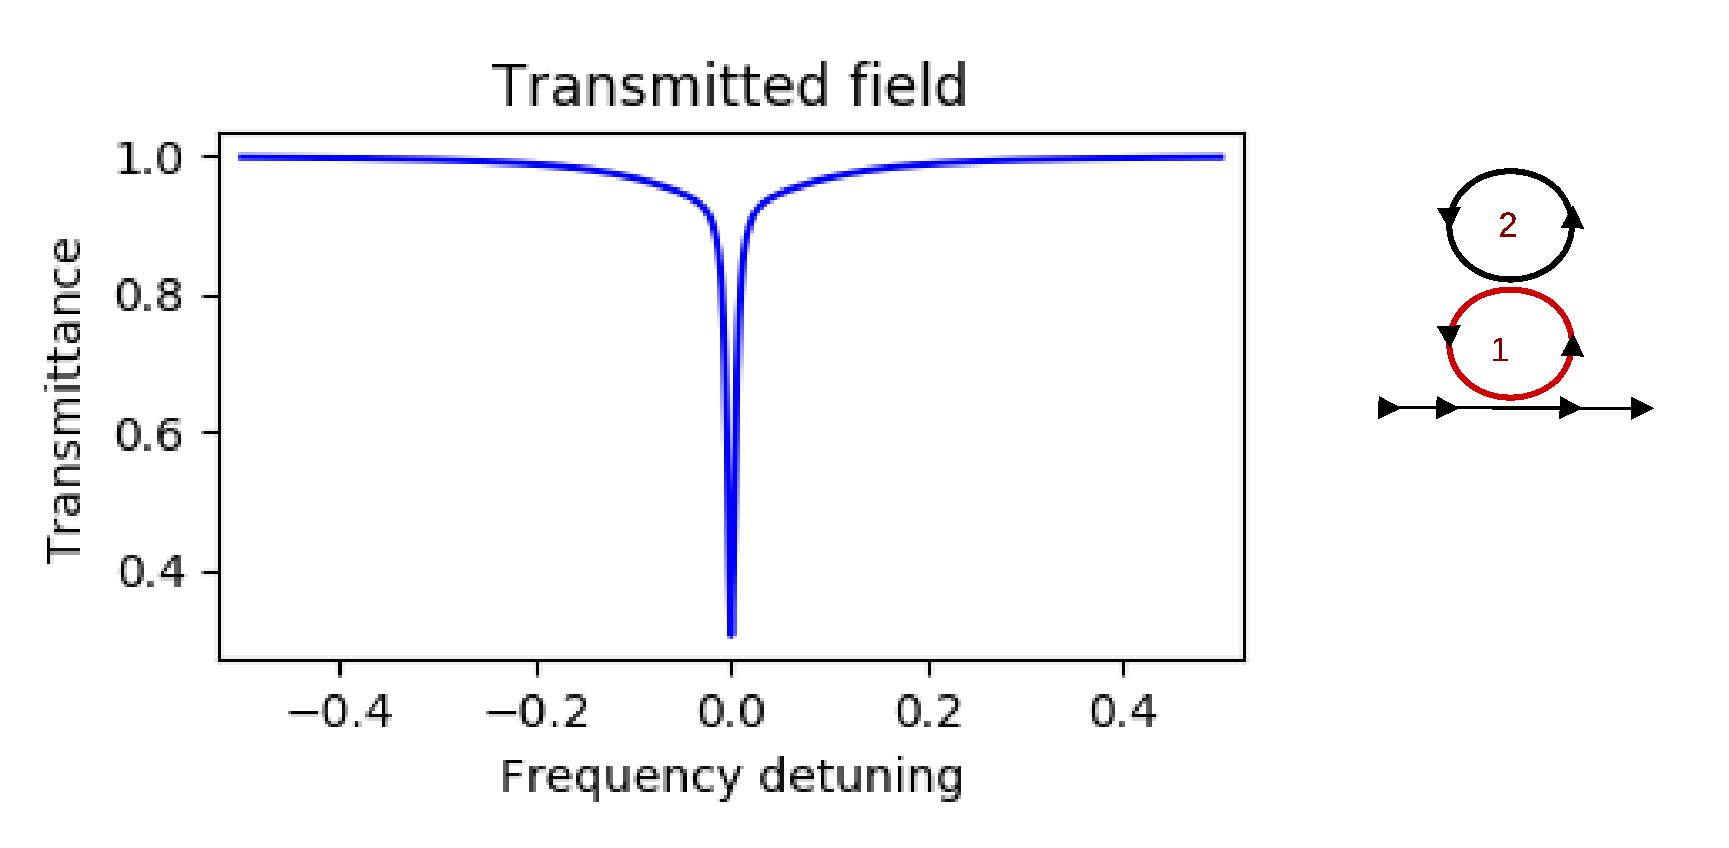
\includegraphics[scale=0.30]{EIA_gain1.eps}
\caption{CRIA with gain activated in first resonator.}
\end{figure}

\begin{figure}[h]
\centering
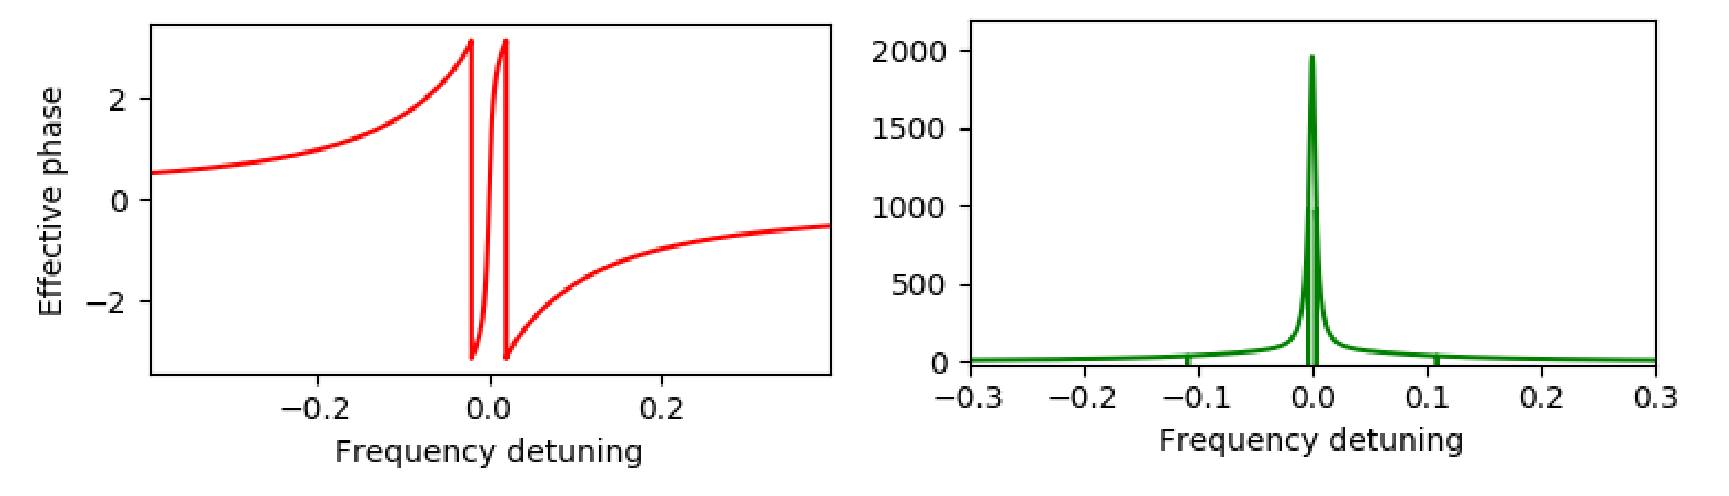
\includegraphics[scale=0.45]{EIA_gain1_phase.eps}
\caption{CRIA phase and group index.}
\end{figure}


\subsection{Introducing Gain In Both Resonators}
Now we consider the case where the gain is activated in both of the resonators simultaneously. No notable changes occurs in the transmission spectrum when $g_{1}$ and $g_{2} < \alpha_{i}$. Fig. 3.20. The phase and group index is also shown in Fig. 3.21.

\begin{figure}[h]
\centering
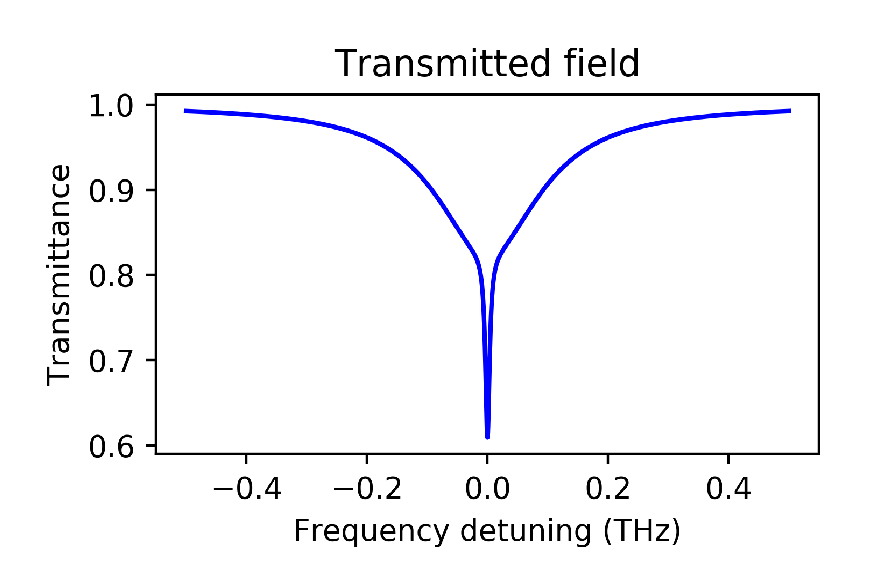
\includegraphics[scale=0.45]{EIA_gain12.eps}
\caption{CRIA with gain in both resonators.}
\end{figure}


\begin{figure}[h]
\centering
\includegraphics[scale=0.5]{EIA_gain12_phase.eps}
\caption{CRIA phase in red and group index in green.}
\end{figure}

However, if gain becomes closer to intrinsic loss, i.e. $g \to \alpha_{i}$, the transmission spectrum values are very near to 1 now and we see anomalous dispersion in the effective phase of the system and negative group index of about $\approx -4550$ (see Fig.3.22).

\begin{figure}[h]
\centering
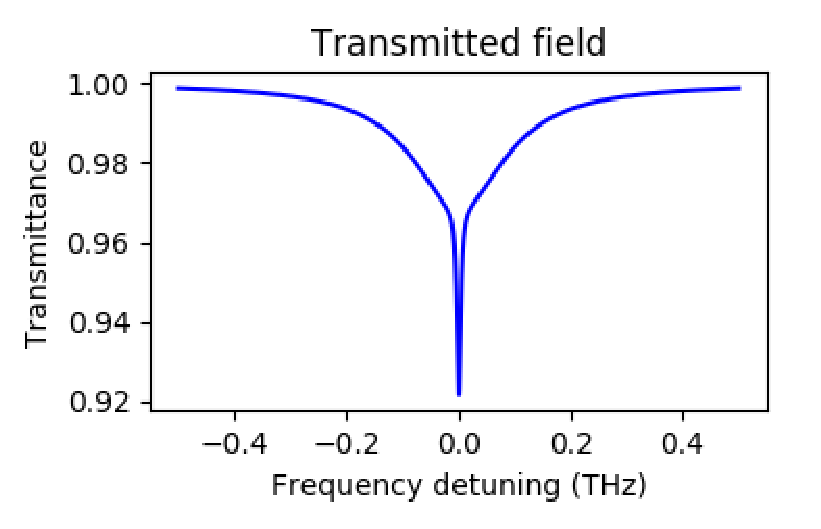
\includegraphics[scale=0.5]{EIA_gain12b.eps}
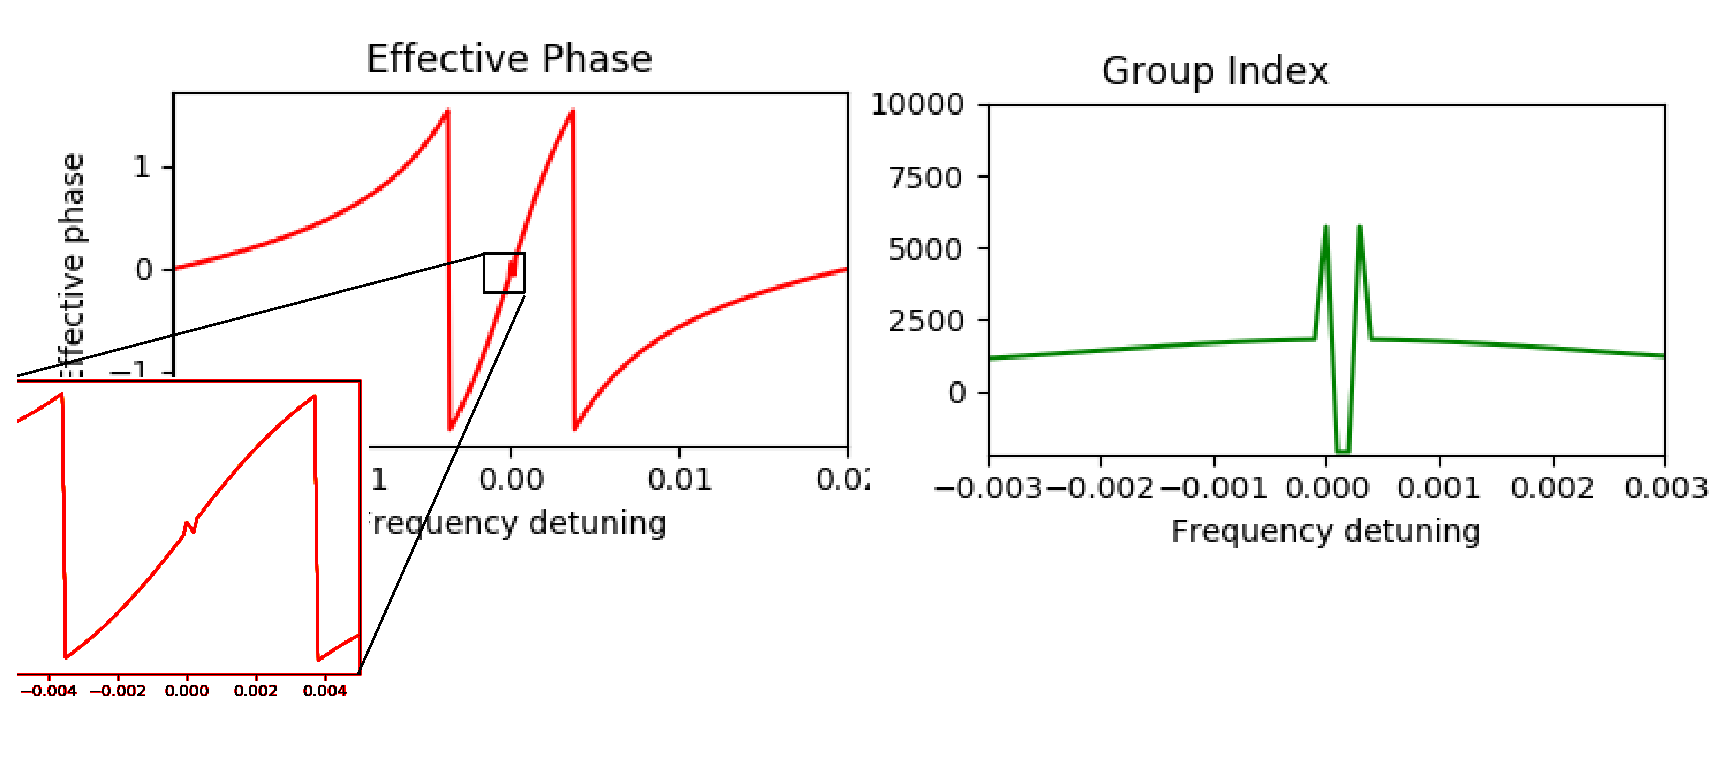
\includegraphics[scale=0.45]{EIA_to_EIT_phase.eps}
\caption{Transmission rises towards unity, dispersion becomes anamolous on resonance, and group index displays negative values.}
\end{figure}

With further increase in the gain, the spectrum flips over the horizontal axis and EIA turns into an EIT like transmission Fig. 3.23. The dispersion remains anomalous as the gain is further increased, i.e. $g > \alpha_{i}$. After the gain achieves a threshold value, again a transition occurs and anomalous dispersion is converted into normal dispersion (Fig. 3.24).

\begin{figure}[h]
\centering
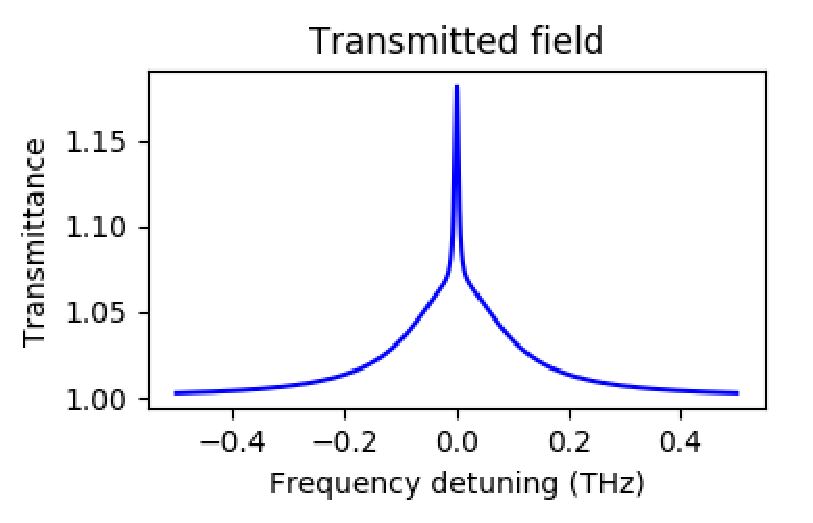
\includegraphics[width=0.40\textwidth]{EIA_gain12ab.eps}
\caption{Transmission of the system}
\end{figure}

\begin{figure}[h]
\centering
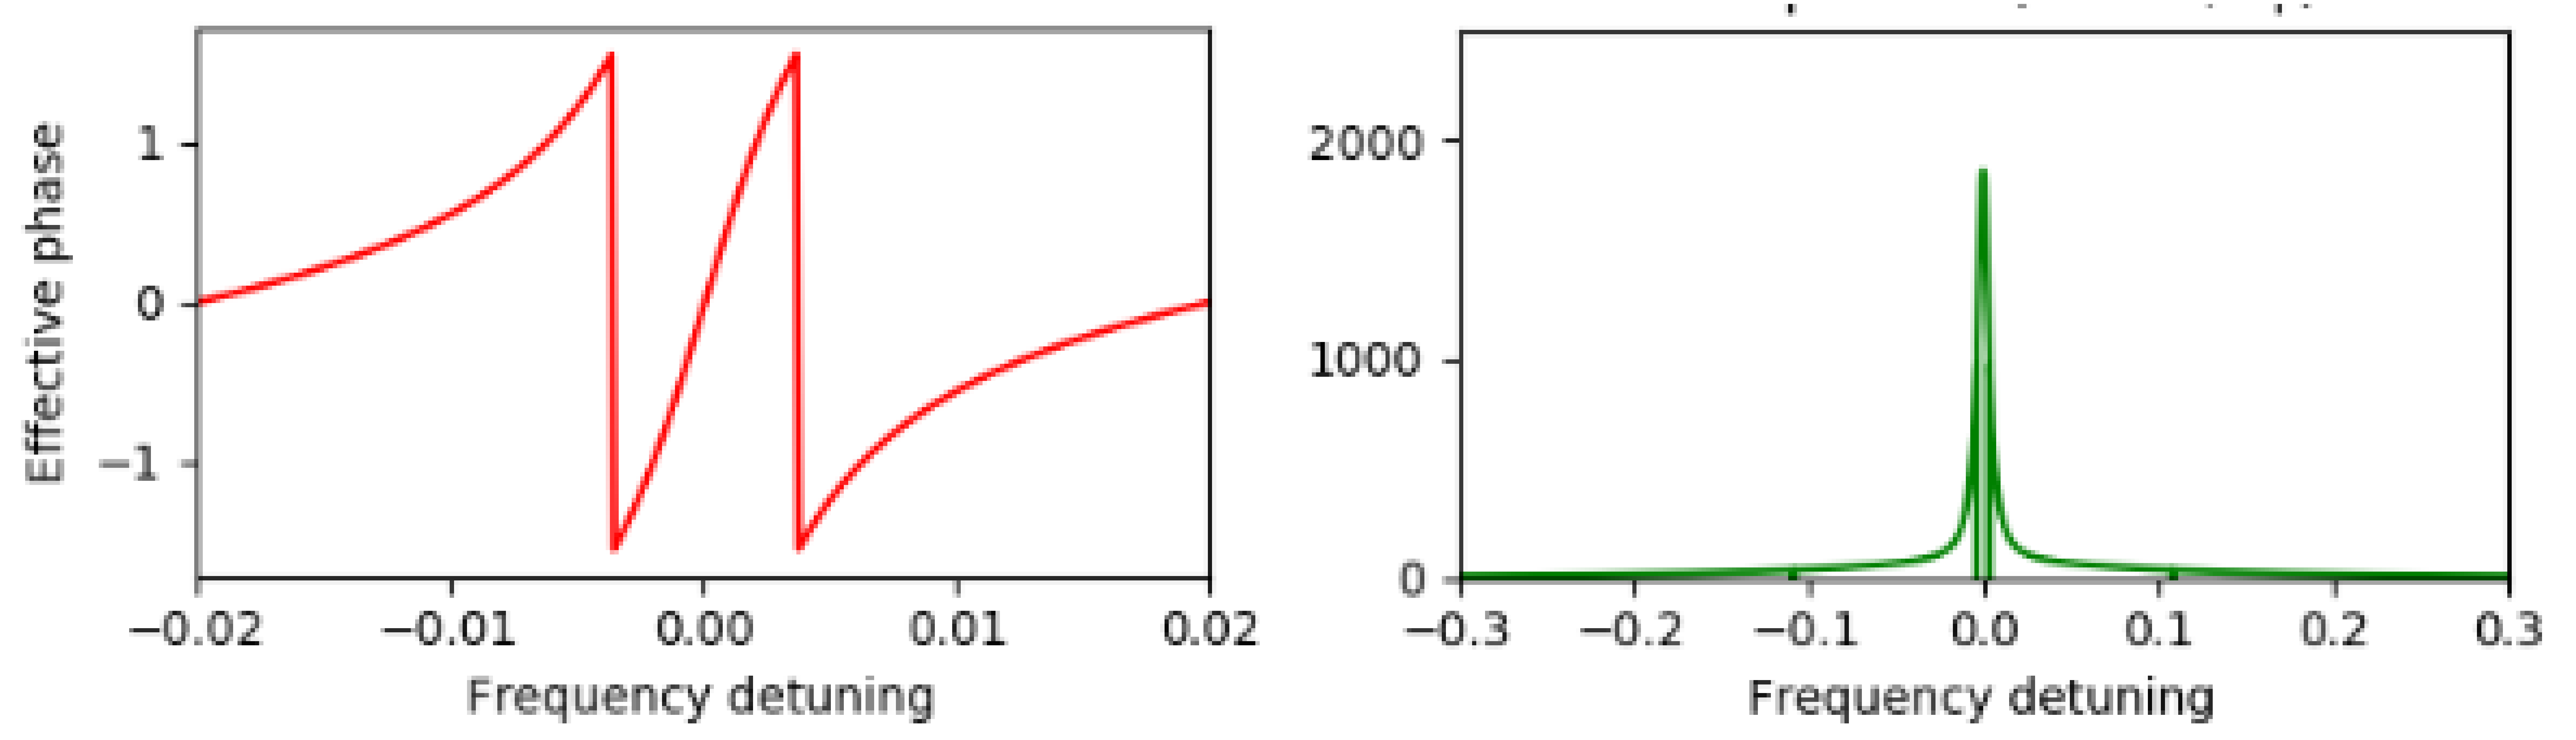
\includegraphics[width=1\textwidth]{EIA_gain_phase1.eps}
\caption{Phase and group index of the system.}
\end{figure}

It is worth noting that the EIT-like resonance shown in Fig. 3.23, usually gives slow light in passive resonators [8]. However, in the present case, fast light is obtained owing to the incorporation of a gain element into the system until a specific threshold gain value.

\subsection{CRIA With Fast Light in Passive Coupled Resonator}
Now we will consider a case featuring CRIA which leads to fast light in a passive coupled resonator system and studies the behavior when the gain is introduced in either one of the resonators. The coupling parameters are given as, $r_{1} = 0.8998$ and $r_{2} = 0.99998$ while the quality factors remains the same. (Fig. 3.25)

\begin{figure}[h]
\centering
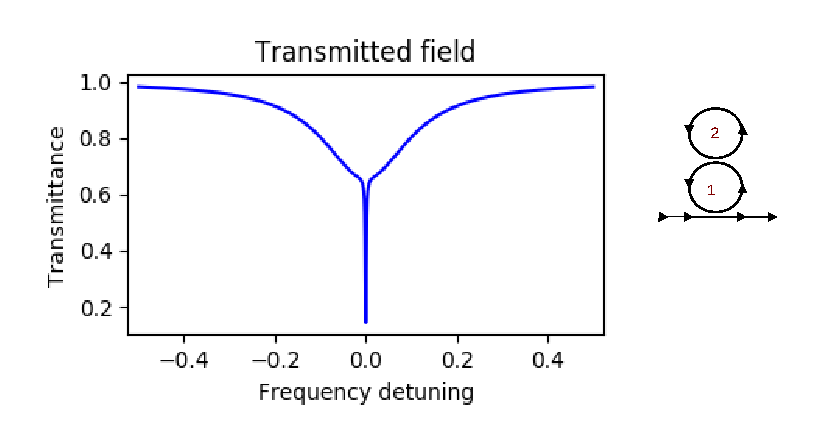
\includegraphics[scale=0.65]{EIAf_passive.eps}
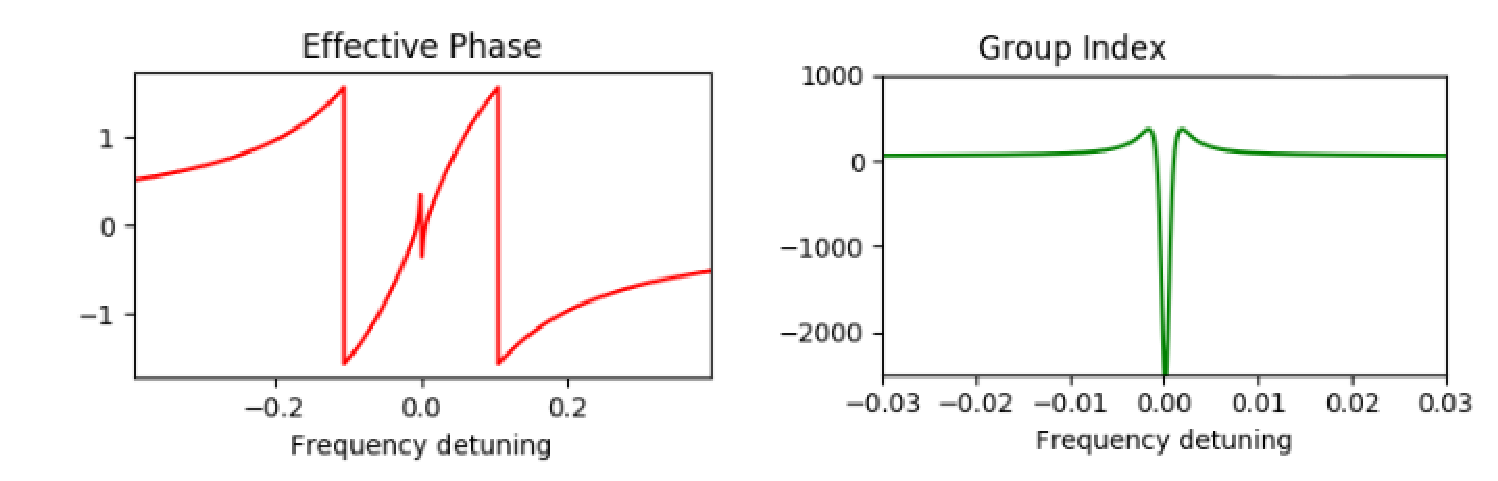
\includegraphics[scale=0.5]{EIAf_passive_phase.eps}
\caption{CRIA observed in a passive two resonator system with anamolous dispersion and negative group index.}
\end{figure}

\subsection{Introducing Gain Only In Second Resonator}
Now we activate gain in the second resonator, shown in the schematic (Fig. 3.26), and observes that the EIA resonance narrows down and becomes sharp. While the amplitude of the narrow CRIA feature decreases, resulting in higher transmission. 

\begin{figure}[h]
\centering 
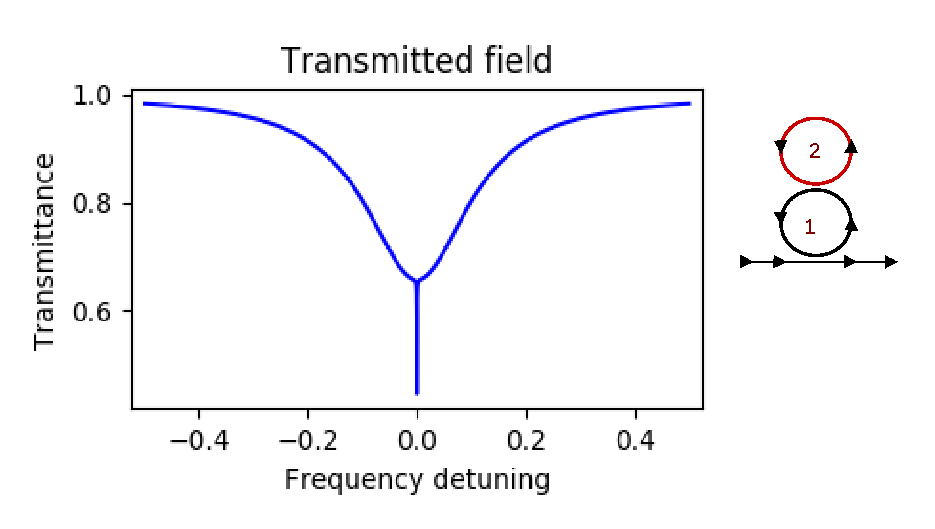
\includegraphics[scale=0.65]{EIAf_gain2.eps}
\caption{Transmission spectrum of CRIA with gain in second resonator.}
\end{figure}


\begin{figure}[h]
\centering
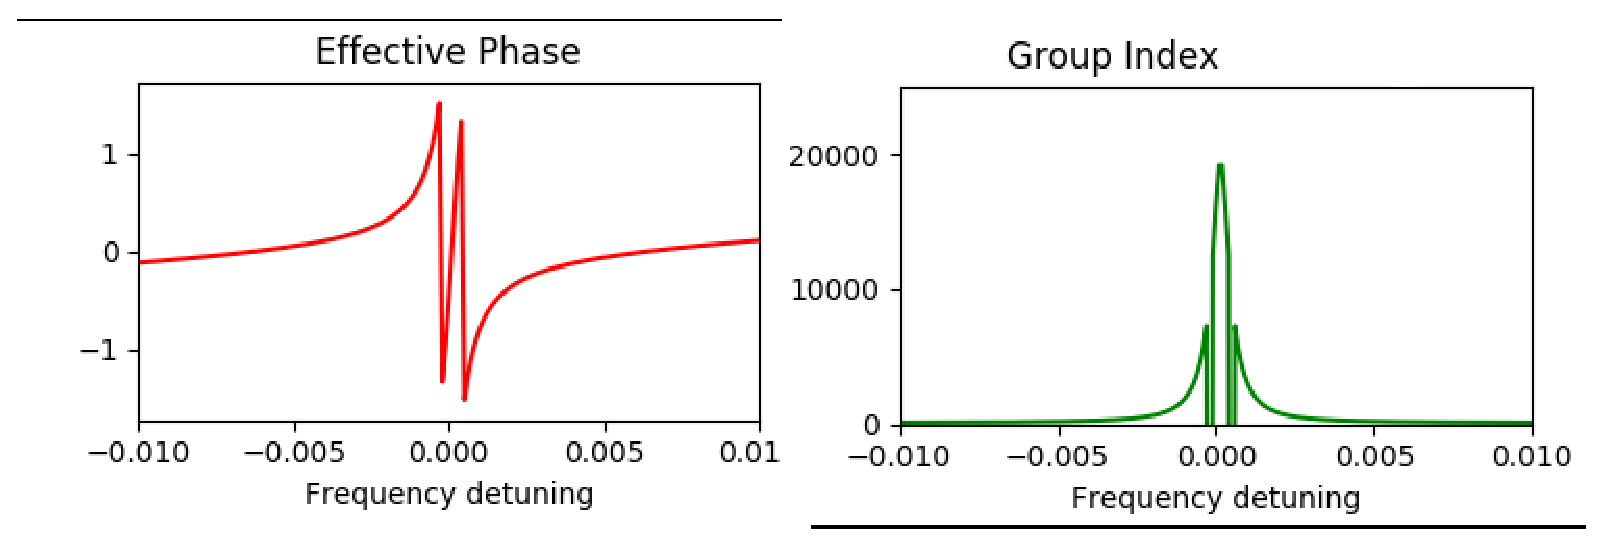
\includegraphics[scale=0.45]{EIAf_gain2_phase.eps}
\caption{Transition from fast to slow light in CRIA.}
\end{figure}

The dispersion of the system changes as gain becomes close to intrinsic loss ($g \approx \alpha_{i}$) and normal dispersion and a positive group index are obtained (Fig. 3.27).

However, when the gain is further increased and it exceeds the intrinsic losses, such that $g > \alpha_{i}$, the spectrum then shows a conversion from CRIA into CRIT (Fig. 3.28) with normal dispersion and positive group index.

\begin{figure}[h]
\centering
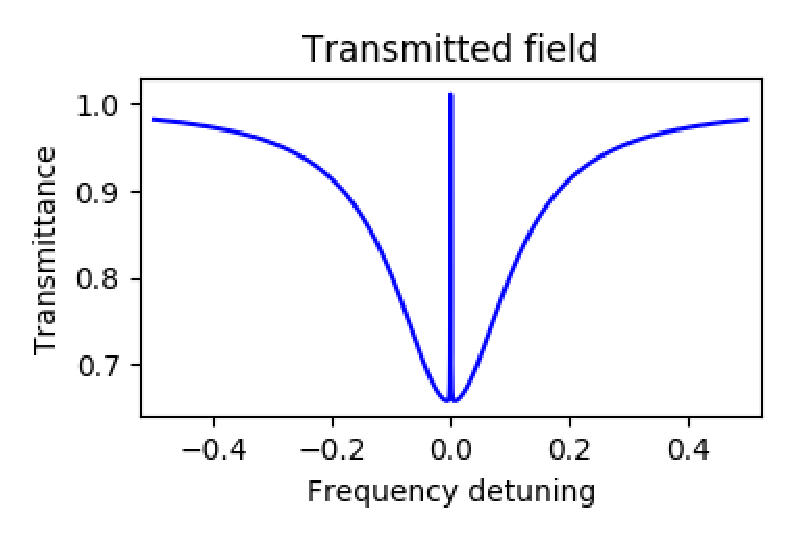
\includegraphics[scale=0.60]{EIAf_gain2a.eps}
\caption{Transmission dip transforming into an tranmission peak.}
\end{figure}

However, the dispersion of the system remains unaffected. It is worth noting that although the dispersion remains subluminal for higher transmission, the transmitted light becomes transparent due to CRIT resonance.

\subsection{Introducing Gain Only In First Resonator}
We again start with the passive CRIA of Fig 3.25. However, now we introduce gain in the first resonator only. We observe the CRIA resonance narrows down and becomes a sharp dip. Also, two off-resonance peaks appear in the spectrum. As $g \approx \alpha_{i}$, the resonance becomes further narrower and the system moves towards critical coupling. We still see fast light and negative group index from here but most of the light is absorbed. The transmission spectrum in Fig. 3.29 is shown for $g > \alpha_{i}$.

\begin{figure}[h]
\centering
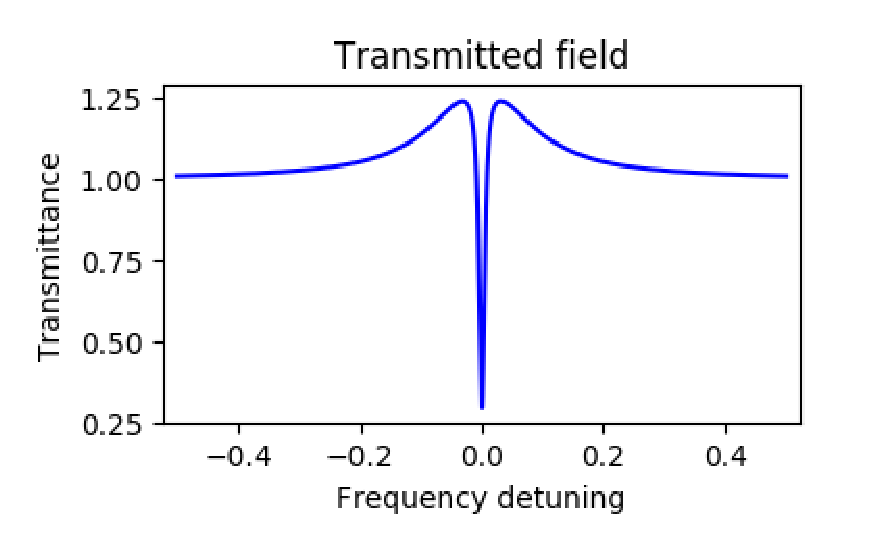
\includegraphics[scale=0.60]{EIAf_gain1.eps}
\caption{Transmission dip of CRIA with gain in first resonator.}
\end{figure}

\subsection{Introducing Gain In Both Resonator}
If we introduce gain in both of the resonators of an initially passive system (Fig. 3.25), simultaneously, we observe the narrowing of CRIA dip and rise of the transmission towards unity. However, the transmission dip changes into a peak when the gain is greater than intrinsic losses ($g > \alpha_{i}$) owing to the transparency of the system (Fig. 3.30). The CRIT resonance of this transparent system leads to normal dispersion and positive group index of $\approx 2\times10^{4}$ (Fig.3.31).

\begin{figure}[h]
\centering
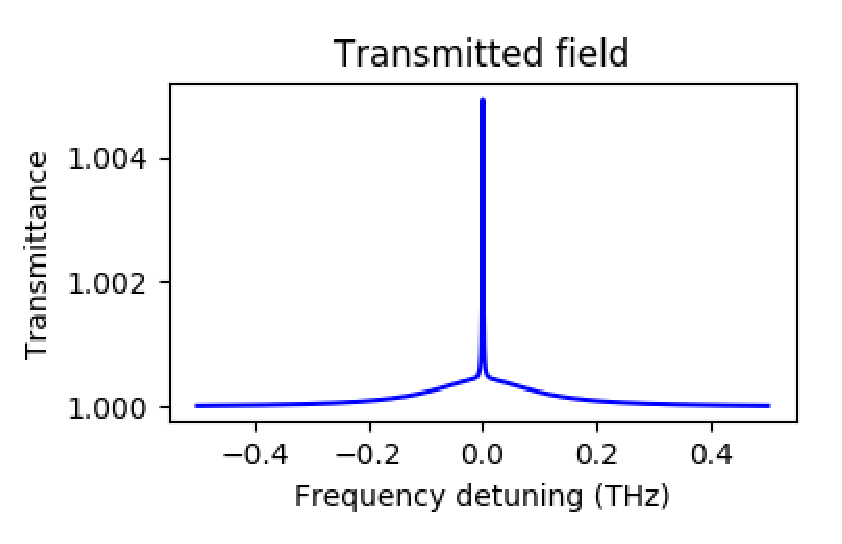
\includegraphics[scale=0.60]{EIAf_gain12.eps}
\caption{Transmission dip transforming into a tranmission peak.}
\end{figure}

\begin{figure}[h]
\centering
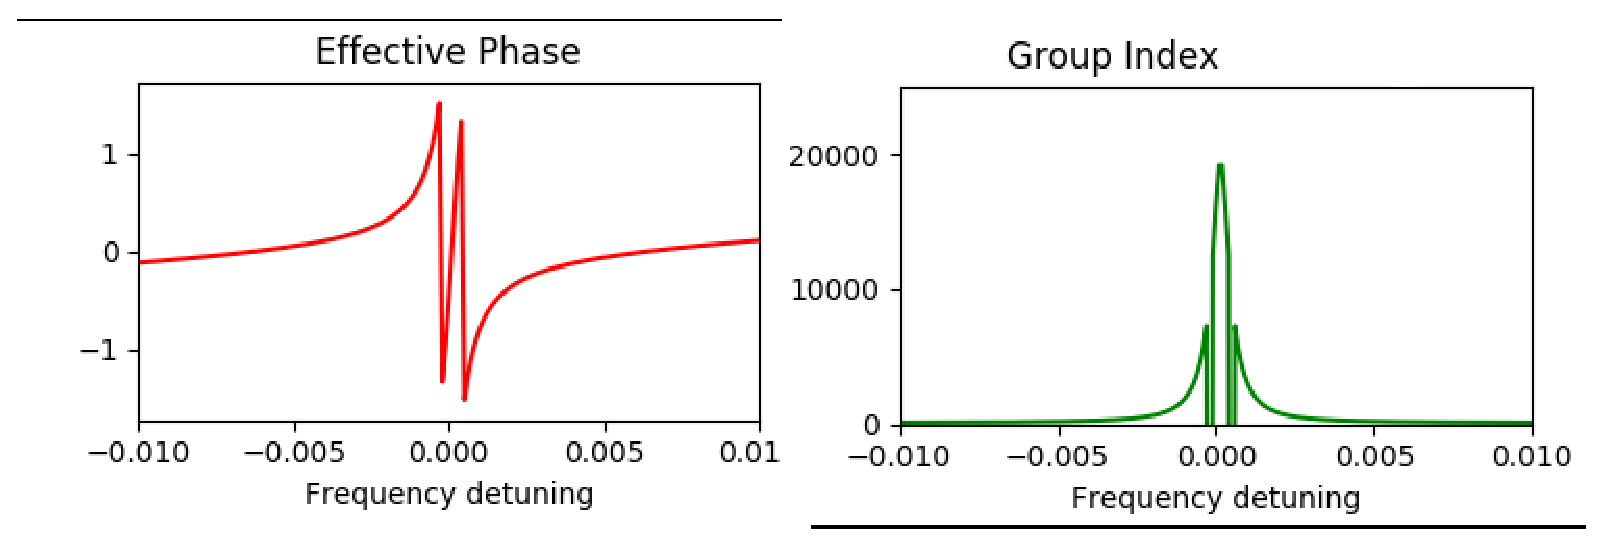
\includegraphics[scale=0.60]{EIAf_gain2_phase.eps}
\caption{Respective phase and group index of the system.}
\end{figure}

These observations lead to the conclusion that when we introduce gain into the system, with it being activated in either one of the resonators or both, we observe drastic changes in the transmission and phase spectrums thus affecting the group delay and dispersion of the system. This allowed achieving gain-assisted tunability of the dispersion of the system, meaning the transitions between fast and slow light can be controlled by simply introducing gain into a passive coupled resonator system.


\section{Proposed Applications}
\subsection{Gain-controlled Optical Pulse Storage and On-demand Retrieval}
Coupling parameter between the two resonators $r_{2}$ can induce very distinct changes into the system.

\begin{figure}[h]
\centering 
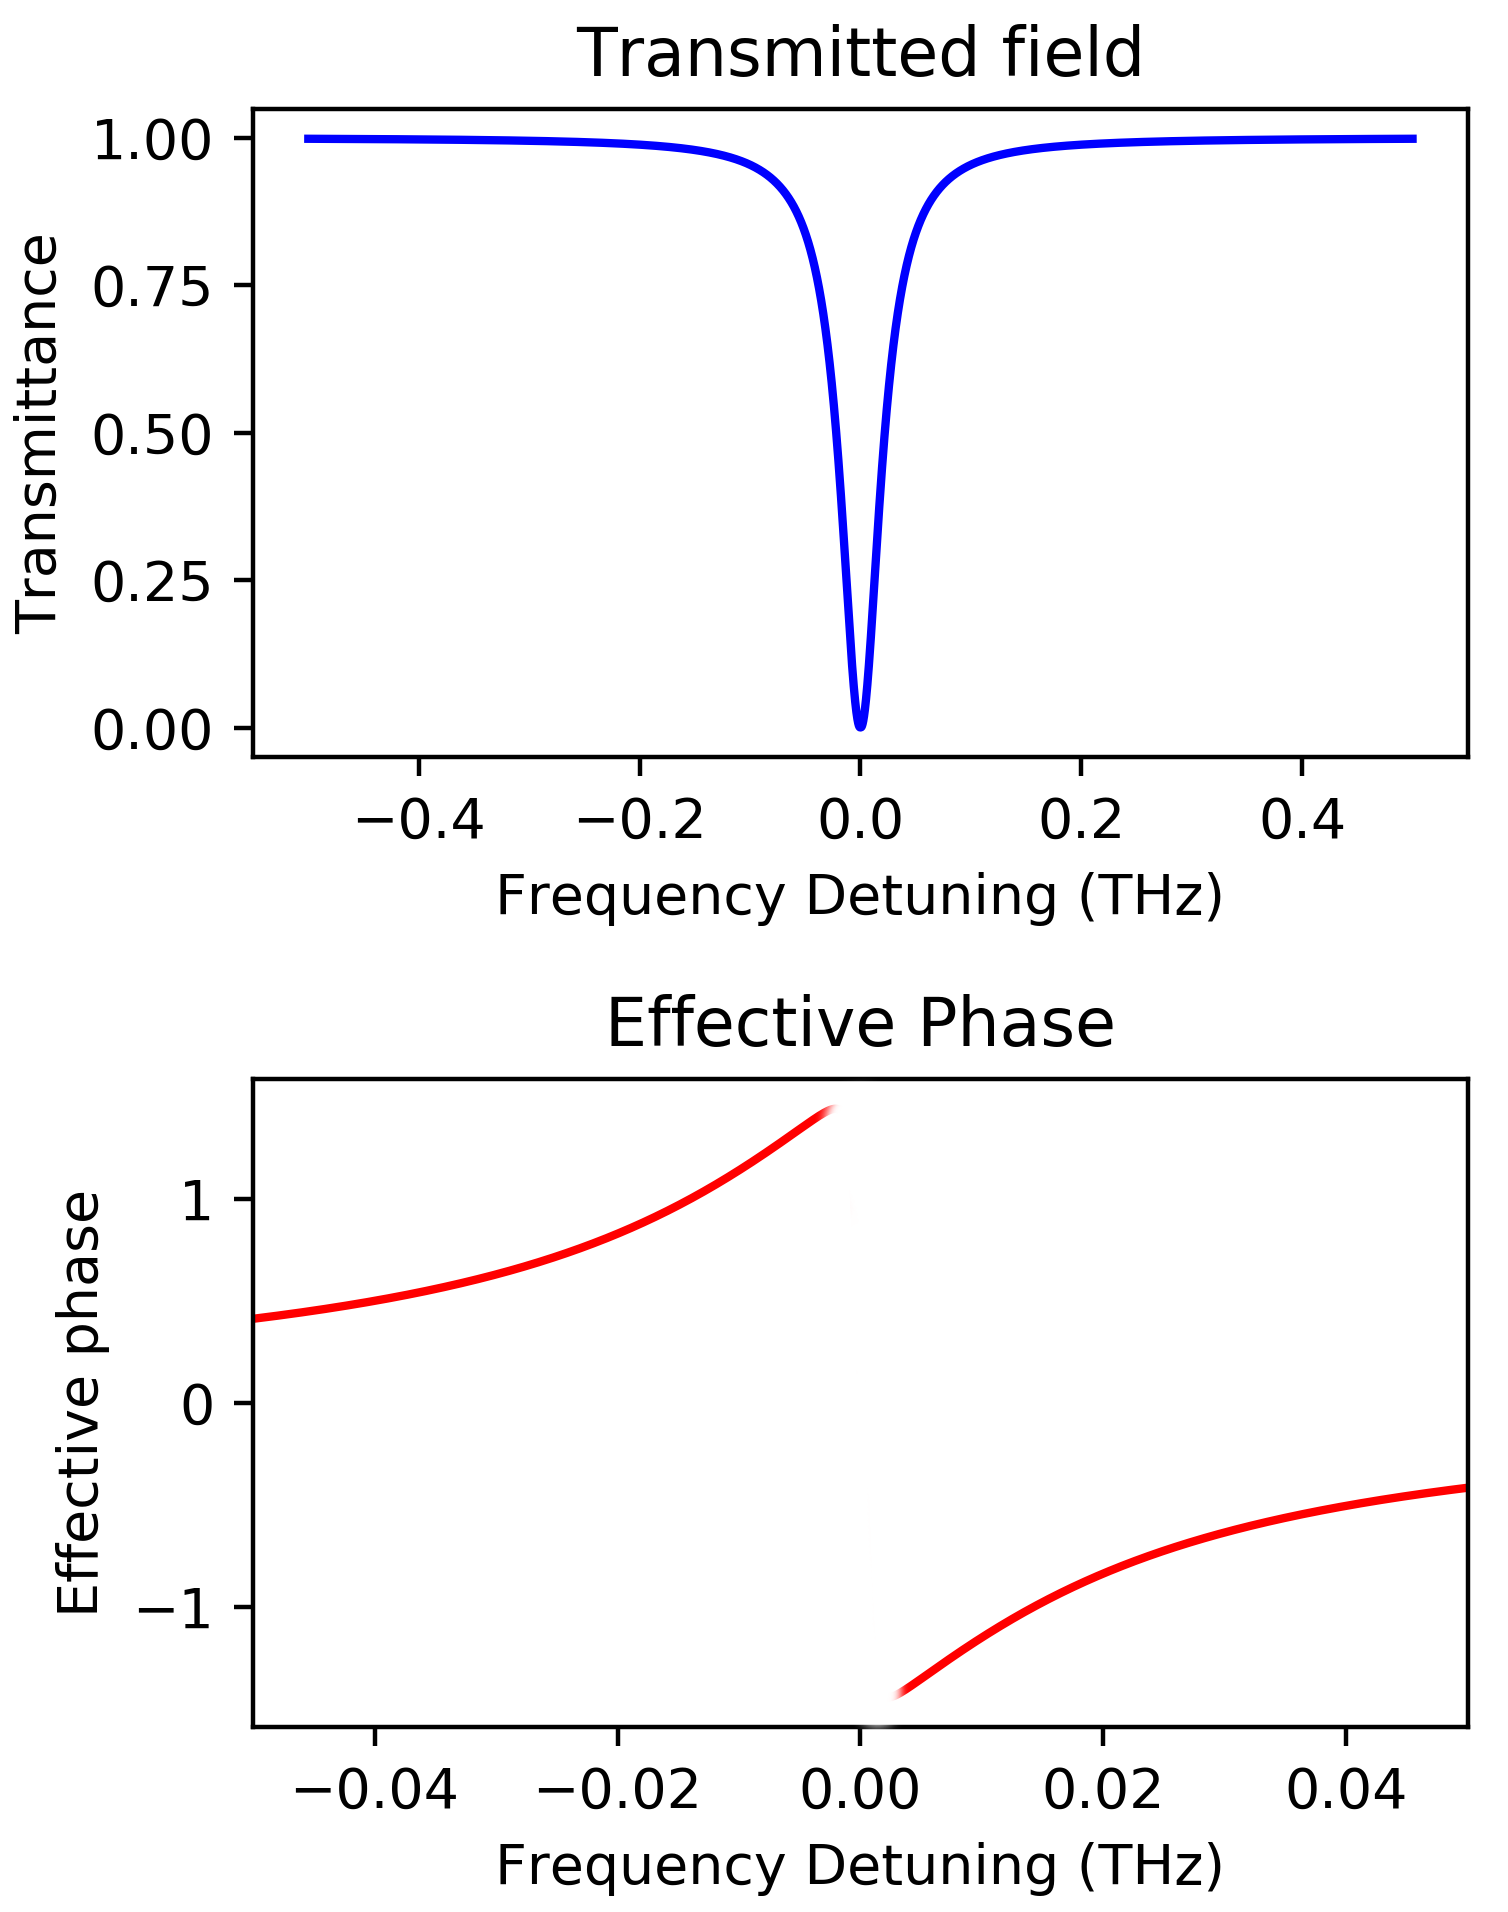
\includegraphics[width=0.5\textwidth]{photon_storage.png}
\caption{Single resonance displayed in a coupled resonator system with its transmission phase.}
\end{figure}

Now we will discuss a case in which the coupling between the two resonators is very weak and the resonance of the second resonator is almost zero. Meaning we have a single resonance transmission at critically coupled i.e. all of the light is absorbed. Fig. 3.32 displays the transmission spectrum along with its effective phase displaying anomalous dispersion. 

Now we will excite gain in the second resonator such that the gain coefficient $g_{2}$, is equal to the intrinsic loss coefficient $\alpha_{i}$. In this state, an input optical pulse whose bandwidth matches the CRIT peak can be coupled to the system. This process happens at nanoseconds scale meaning we can switch from zero to maximum intensity in nanoscale durations. Fig. 3.33 displays the gain excited transmission with normal dispersion meaning we have slow light which was the main ambition.

This shows that the light pulse is now stored inside the coupled resonator system and to retrieve the stored pulse back. As soon as the light pulse has entered the system, the gain is turned off. Once again a critically coupled transmission resonance appears in the spectrum. The true shape of the input signal is not disturbed the narrow peak of EIT shows us that very narrow bandwidth of frequencies can be stored. For this case, a narrow bandwidth pulse can be stored in a coupled-resonator. However, by using a lower-Q second resonator a larger bandwidth pulse can be stored.

\begin{figure}[h]
\centering 
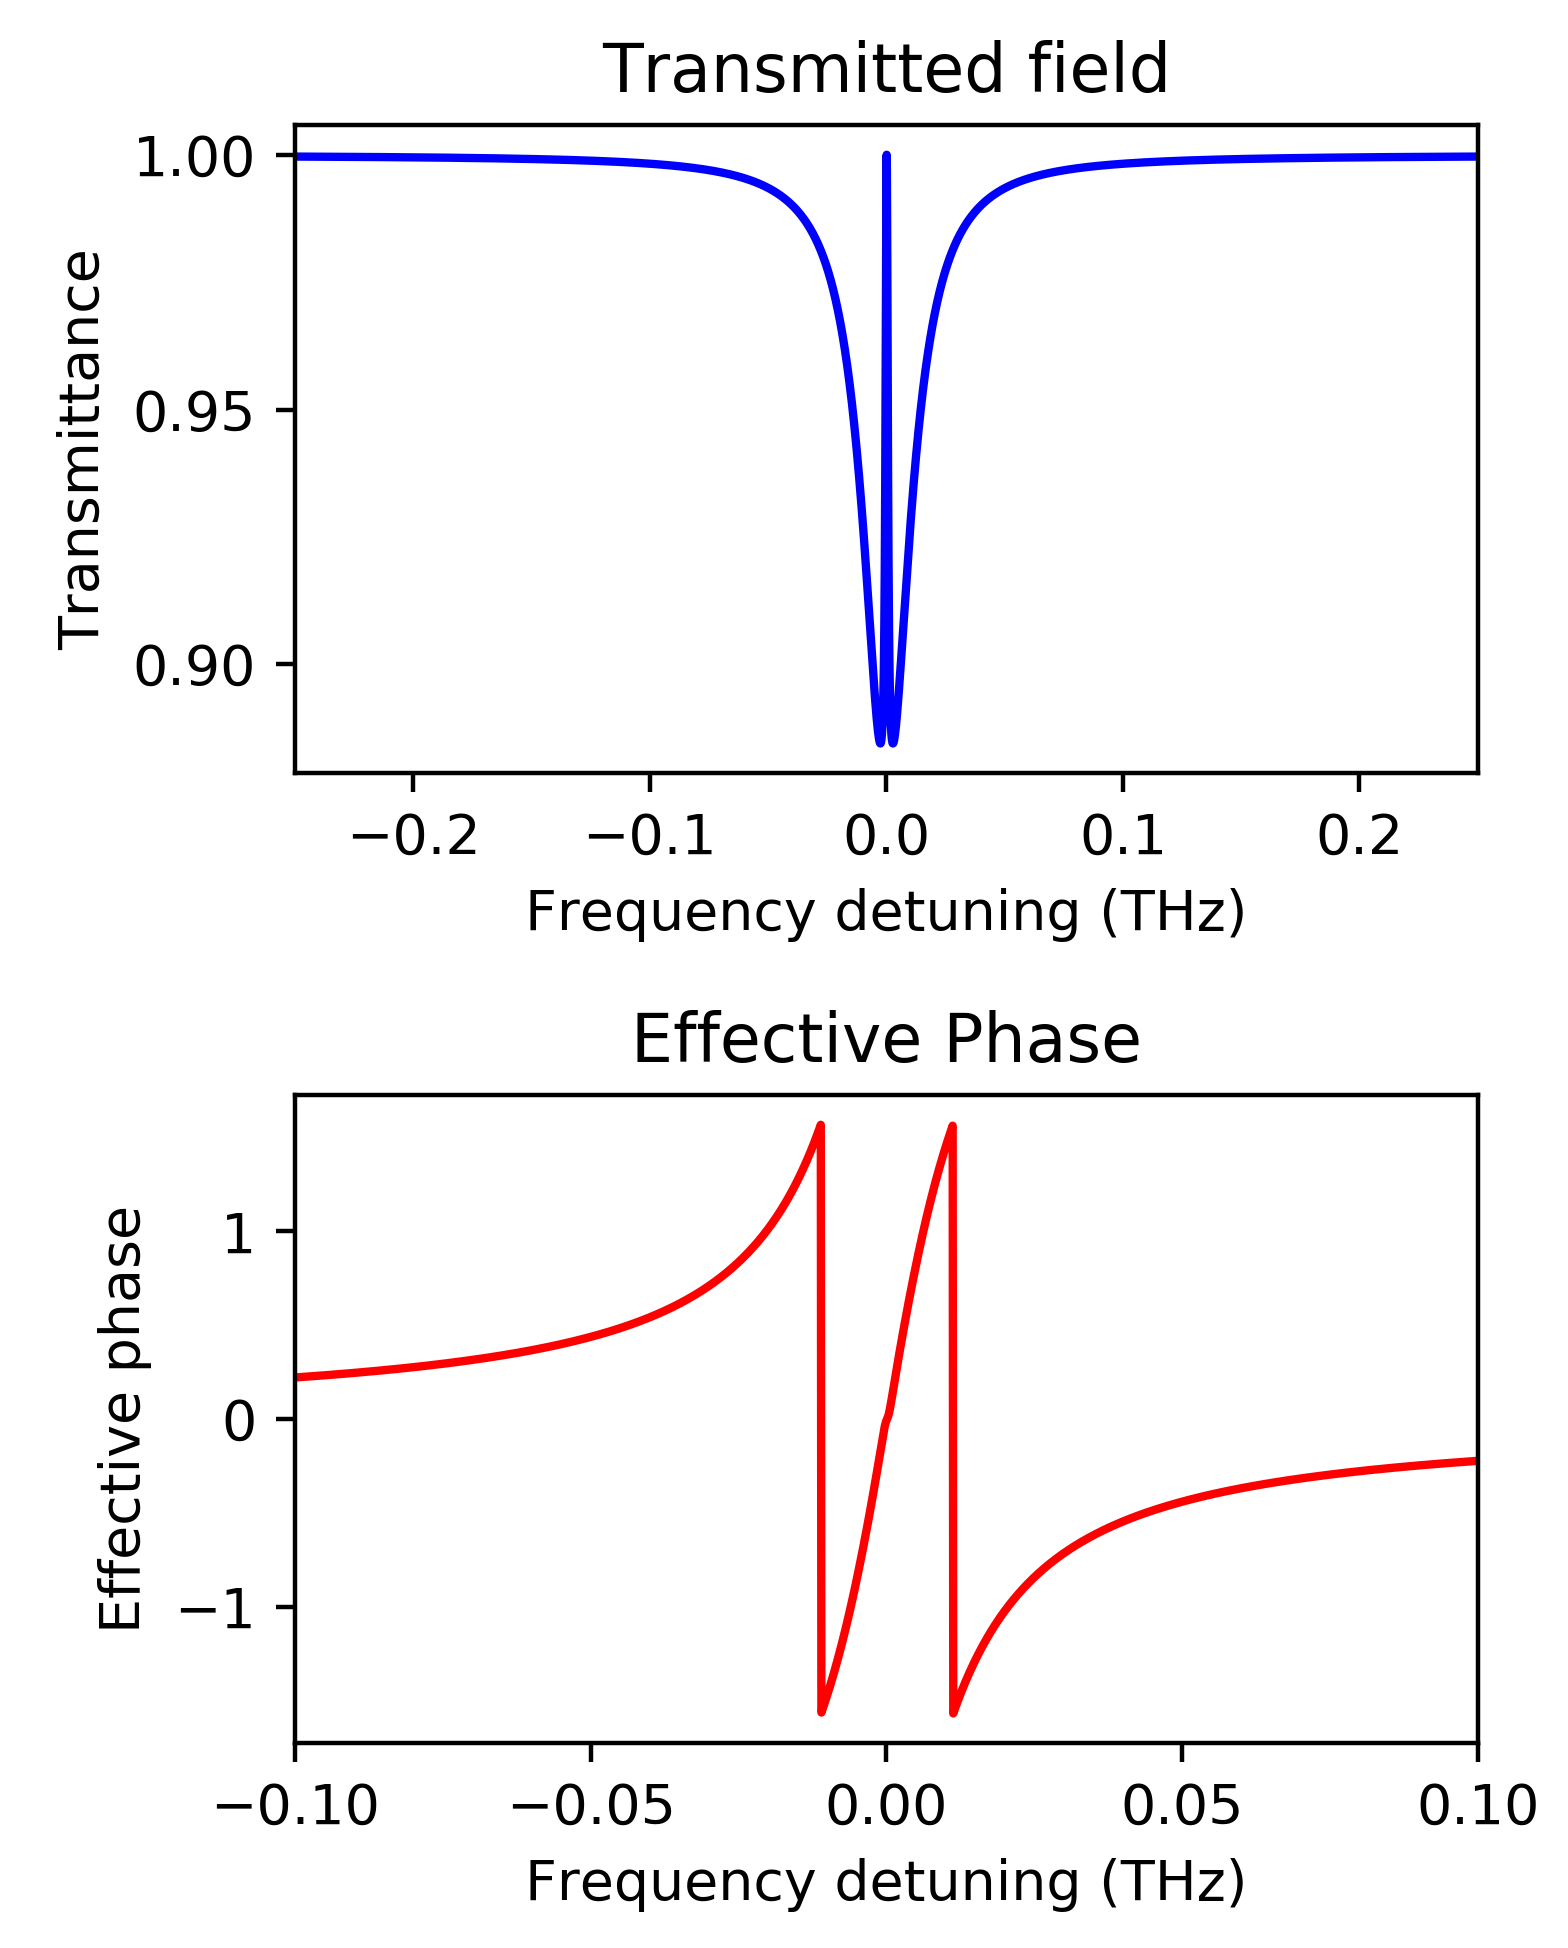
\includegraphics[width=0.50\textwidth]{photon_storage_gain.png}
\caption{EIT peak emerges when gain is excited in second resonator in a coupled resonator system. The corresponding transmission phase is also shown.}
\end{figure}

\subsection{Gain Controlled Slow and Fast Light Tuning}
We have observed from these results that the transitions from super and subluminal velocities of light have been in the control of the optical gain of the system. We have observed superluminal regimes of transmission reverting into subluminal transmission by the excitation of gain in either one or both coupled two resonator system. Also, the subluminal transmissions such as EIT which always displays slow light in passive systems provided us with fast light and anomalous dispersion in the presence of gain in either of the resonators. This tuning of gain made possible the transitions between fast and slow light in both ways, meaning we have achieved control over how and when do we want fast and slow light for our device.

\newpage
\section{Discussion}
We showed tunability of optical analogs of Electromagnetically Induced Transparency (EIT) and Electromagnetically Induced Absorption (EIA). This enabled pulses that propagate through system owing to controlled excitation of the gain medium. superluminal and subluminal group velocities of light in a coupled ring resonator framework, with a direct increase excitation and empowered reversible advances between them. Besides, we watched sub and superluminal light including all-optical EIT reverberation, which in every single past examination, given inactive coupled ring resonators, has been seen to yield just subluminal light. In addition to control of sub and superluminal group velocities, we observed a CRIT resonance which displays fast light. It is worth noting that CRIT in all previous studies focusing on passive coupled resonators always led to slow light. 


\newpage
\section*{References}
\addcontentsline{toc}{section}{References}

\paragraph{\normalfont \large $[1]$ S. H. Autler and C. H. Townes, “Stark effect in rapidly varying fields,” Phys. Rev. \textbf{100} (1955). \\ 
\\$[2]$ S. E. Harris, “Electromagnetically Induced Transparency" Physics Today, July 1997. \\
\\$[3]$ D. D. Smith, H. Chang, K. A. Fuller, A. T. Rosenberger, and R. W. Boyd, “Coupled-resonator-induced transparency,” Phys. Rev. A \textbf{69}, 063804 (2004). \\
\\$[4]$  A. Naweed, G. Farca, S. Shopova, and A. T. Rosenberger, “Induced transparency and absorption in coupled
whispering-gallery microresonators,” Phys. Rev. A \textbf{71} (2005).\\
\\ $[5]$ B. Peng, S. K. Ozdemir, W. Chen, F. Nori, L. Yang “What is and what is not electromagnetically induced transparency in whispering-gallery microcavities", Nature. Comm. \textbf{5}:5082 (2014).\\
\\ $[6]$ Y.C. Liu, B.B. Li, and Y.F. Xiao “Electromagnetically induced transparency in optical microcavities", nanoph-2016-0168, (2017).\\
\\ $[7]$ S. Zhu, L. Shi, S. Yuan, R. Ma, X. Zhang and X. Fan, “All-optical controllable electromagnetically induced transparency in coupled silica microbottle cavities", nanoph-2018-0111 (2018).\\
\\ $[8]$ A. Naweed, “Photonic coherence effects from dual-waveguide coupled pair of co-resonant microring resonators", Opt. Exp. \textbf{23} (2015).\\
\\ $[9]$ K. Totsuka, N. Kobayashi, and M. Tomita, “Slow light in coupled-resonator-induced transparency,” Phys. Rev.
Lett. \textbf{98}(21), 213904 (2007).}